\cotefile{156-4}
\scanpage{2}
\mspage{1}
\margin{\begin{tabular}{|l}\unsure{GF|CF} $\overline{\underline{\mathrm{IV}}}$\\\hline\end{tabular}}
\uline{Analysis situs} (première mouture).

(10 juin 1986)

1. Comme modèle ``ensembliste topologique de l'axiomatique d'un ``modèle de \unsure{formes|forme} \inserted{topologiques}'' (cas d'une ``\uline{\unsure{contrée}}''),
considérons les notions \unsure{suivantes} \unsure{Modèle} : un ``espace'' $\pm$ \unsure{ordinaire} $\deleted{\unsure{X}}\unsure{E|X}$.
On \unsure{suppose|supposera} ici que $\deleted{X}E$ \unsure{est} un espace topologique séparé, \unsure{ou} un espace modéré (pas néc. compact) pour une théorie \unsure{modérée} donnée.

Dans ce cas ``partie fermée'' signifie ``partie fermée \unsure{modérée}''

I) \uline{Figure} \qquad Une \uline{figure} \inserted{$F$} de $\deleted{X}E$ est une partie fermée $X$, \uline{munie} d'une
% slanted
\margin{$X$ est appelé le \uline{support} de la figure $\operatorname{supp} F$ ou $\lvert F\rvert$}
décomposition de $Y$ en \deleted{\unsure{strates}} \inserted{parties} $X_i$
\[
\{X_i\}\in\mathcal{P}(Y) \qquad X=\bigcup X_i
\]
appelées les \uline{strates fermées}. On fait les hypothèses

a) Les $X_i$ fermés \inserted{non vides et loc. compacts (loc. \unsure{cpt|cpt.} est \unsure{autom.} si $\deleted{X}E$ l'est, par ex. \unsure{Esp. mod.})} (pas néc. compacts \unsure{\}} \deleted{\unsure{mais}} \unsure{ils le s\textsuperscript{t}} si $X$ l'est\unsure{)}

b) La famille des $X_i$ est loc. finie
\inserted{(donc par a) b) \unsure{d'où|d} $\Rightarrow$ réunion \unsure{de|des} str.~f. est fermée\unsure{)}}
\margin{NB on pose $i\leq j\iff X_i\subset X_j$ \quad $i<j\iff X_i\unsure{\subsetneqq|\nsubseteq}X_j$}

c) Si \deleted{\unsure{$X_i=$}} \deleted{\unsure{$\partial X_i=$}} $X_i\subset X_j$, $X_i\ne X_j$, (i.e. $i<j$) alors $X_i$ \uline{rare} dans $X_j$

d) Posant $\partial X_i=\deleted{\unsure{\bigcup_{X_j\subsetneq X_i}X_j}}\bigcup_{j<i}X_j$ (donc $\partial X_i$

\scanpage{3}
\mspage{2}
est fermé rare en $X_i$, par a) b) c)) \deleted{\unsure{est}} $\operatorname{int}(X_i)=X_i\setminus\partial X_i$, lequel est donc un ouvert \inserted{rel.} dense de $X_i$, et non vide puisque $X_i$ l'est) est \deleted{\unsure{une}} 1\textsuperscript{o}) \uuline{variété} 2\textsuperscript{o}) \uline{connexe}. (NB dans le cas $E$ modéré, on prend ``variété'' au sens modéré, certes.)
% slanted
\margin{e) Si $\deleted{X_i<X_j}\inserted{i<j}$ alors $\dim\unsure{\text{l'int}|\operatorname{int}|\operatorname{ind}}(X_i)<\dim\unsure{\operatorname{int}|\operatorname{ind}}(X_j)$, pour éviter des phénomènes de sauvagerie}
% slanted; orient the marginal drawing as on the sheet
\figure{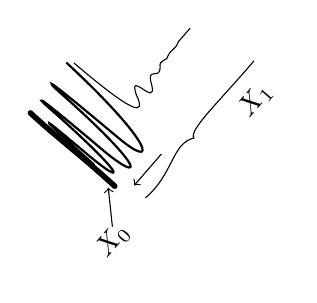
\begin{tikzpicture}[x=.85cm,y=.85cm]
\begin{scope}[rotate=49]
\draw[line width=2pt,line cap=round] (0,0) .. controls (.02,.7) and (-.02,1.15) .. (0,1.67);
\draw[line width=.8pt] (.04,.44) .. controls (.055,1.57) and (.075,1.67) .. (.09,.68)
 .. controls (.10,-.20) and (.23,-.04) .. (.24,1.60)
 .. controls (.26,1.87) and (.28,1.30) .. (.29,.49)
 .. controls (.31,-.34) and (.51,-.17) .. (.52,1.64)
 .. controls (.54,1.88) and (.56,1.58) .. (.58,.46)
 .. controls (.59,-.35) and (.86,-.05) .. (.92,1.76);
\draw (.99,1.67) .. controls (1.00,.48) and (1.10,.33) .. (1.24,.65)
 .. controls (1.45,1.01) and (1.29,.29) .. (1.50,.57)
 .. controls (1.67,.84) and (1.62,.53) .. (1.78,.65)
 .. controls (1.87,.76) and (1.93,.62) .. (2.00,.68)
 .. controls (2.11,.71) and (2.16,.65) .. (2.25,.70) -- (2.52,.70);
\draw[<-] (.20,-.21) -- (.82,-.21);
\draw (.17,-.46) .. controls (.72,-.54) and (1.05,-.22) .. (1.32,-.42)
 .. controls (1.34,-.28) and (2.00,-.35) .. (2.78,-.34);
\draw[->] (-.48,-.37) -- (-.08,.06);
\node[rotate=49] at (-.63,-.51) {$X_0$};
\node[rotate=49] at (2.35,-.74) {$X_1$};
\end{scope}
\end{tikzpicture}}

\deleted{\unsure{e}}f) $X_i\cap X_j$ est réunion \unsure{de|des} $X_k$.

Donc une figure \inserted{$F$} peut s'identifier à l'ens de ses strates, qui est un ens de parties fermées de $X$
\[
\underset{\substack{\shortparallel\\\{X_i\}}}{F}\subset\mathcal{P}_f(x)
\qquad \text{i.e.}\qquad F\in\mathcal{P}(\mathcal{P}_f(X))
\]
($X$ se réconstitue comme $\bigcup X_i$), satisfaisant certaines conditions \inserted{(qu'on vient d'expliciter, a) à d))}. On a donc l'ens des figures, \deleted{qui} soit $\mathcal{F}$, qui est donc un ens. de parties de $\mathcal{P}_f(x)$
\[
\mathcal{F}\subset\mathcal{P}(\mathcal{P}_f)\qquad\text{i.e.}\qquad
\mathcal{F}\in\mathcal{P}(\mathcal{P}(\mathcal{P}_f(X\unsure{)))|))}
\]

À chaque $F\in\mathcal{F}$ est associé \uline{l'ens ordonné} $\Sigma_F$ de ses strates. L'ens somme
\diagram{\begin{tikzcd}[ampersand replacement=\&,column sep=small,row sep=small]
\Sigma \arrow[d,"{\rule{16mm}{.25pt}}"'] \& {}=\displaystyle\coprod_{F\in\mathcal{F}}\Sigma_F\\
\mathcal{F} \&
\end{tikzcd}}
{\reversemarginpar\margin{les fibres sont les $\Sigma_F$}}
\margin{\uline{NB} Dans le cas d'espèce, on \unsure{à|a} $\Sigma_F\equiv F$, \deleted{\unsure{mais l'ai|mais j'ai} \illegible{1} \unsure{déjà|dit}.}}
peut aussi s'identifier à l'ens des couples $(F,X_i)$, \deleted{$F$ e} où $F$ est une figure et $X_i$ est une strate de $F$ i.e. $X_i\in F$.

\scanpage{4}
\mspage{3}
Si $F,F'$ sont deux figures, on dit que $F'$ est une \uline{sous-figure} de $F$, si \unsure{toute|tout} strate de $F'$ est une strate de $F$, i.e. $F'\subset F$. Donc \deleted{le support} on aura \deleted{\unsure{$\sigma(F)$}} \unsure{d|et} $\lvert F'\rvert\subset\lvert F\rvert$

\uline{NB} Si $X_i\in F'$, et $Y_j\in F$ est tel que $Y_j\subset X_i$, alors $Y_j\in F'$

\deleted{En effet, soit $y\in\deleted{\unsure{Y_j}}\operatorname{int}(Y_j)$, alors}

\deleted{La relation}

On écrit $F'\leq F$ pour cette relation, qui est une relation d'ordre dans $\mathcal{F}$.

L'ens des sous-figures de $F$ est en corr. 1-1 avec l'ens des parties \inserted{$\Phi$ ($=\Sigma_{F'}$)} de \deleted{\unsure{$F$|$\mathcal{F}$}} \inserted{$\Sigma_F$, (ens des strates)} qui ont la \unsure{propriét.|propriété} que \inserted{$i,j\in\Sigma_F$,} $i\in\deleted{\unsure{\Sigma|B}}\Phi$, $j\leq i\Rightarrow j\in\Phi$
(\deleted{idéaux} \inserted{``\unsure{fermées|fermés}''} \deleted{fermés} de l'ens \deleted{\unsure{ens}} ordonné, pour la top. \inserted{sur $\Sigma_F=\Sigma$} \unsure{ayant} comme base \deleted{de fermés} \deleted{d'ouverts \unsure{/} les} \inserted{d'ouverts les} $\Sigma_{\deleted{\unsure{>}}\unsure{\geq|\leq}i}$).

\deleted{\unsure{Ainsi|$F'\leq F$}, on a une relation d'ordre sur}
% slanted
\margin{\uline{11.6.} Je dirai plus tôt ``\uline{multistrate}''}

\uline{Figure élémentaire} : qui a une strate maximale i.e. $\Sigma_F$ a un plus grand élément. Soit \tikz[baseline=(el.base)]{\node[inner sep=1pt] (el) {$\mathcal{F}_{\text{él}}$};\draw (el.center) ellipse [x radius=1.05em,y radius=.78em];} l'ens des figures élémentaires. \deleted{Alors} Pour tte figure $F$, les sous-figures élémentaires sont en corr 1-1 avec les

\scanpage{5}
\mspage{4}
strates de $F$. \deleted{Donc on peut \unsure{ide|idé}}
\[
\begin{aligned}
 F &\quad \text{figure}\\
 \Sigma_F &\quad \text{ens de ses strates}\\
 \Sigma'_F &\quad \text{ens des sous-figures élémentaires.}
\end{aligned}
\]
On :
\diagram{\begin{tikzcd}[ampersand replacement=\&,column sep=small,row sep=.35em]
\Sigma'_F \& {}\simeq\Sigma_F\\
{\unsure{\rotatebox{-90}{$\subset$}|\cap|\rotatebox{-90}{$\in$}}} \&\\
\mathcal{F}_{\text{él}} \&
\end{tikzcd}}
$F$ est connu quand on connait $\Sigma'_F\subset\mathcal{F}_{\text{él}}$ car $F$ est l'ens des strates des $F'\in\Sigma'_F$.

Mais la relation d'inclusion entre figures \unsure{s'interprete|s'interprète} comme relation d'inclusion entre \unsure{partie|parties} de $\mathcal{F}_{\text{él}}$.

\deleted{Deux f}

Considérons la relation d'inclusion \inserted{$\leq$} entre figures élémentaires. \deleted{\unsure{A}}Alors, $\mathcal{F}_{\text{él}}$ est un ens ordonné. \deleted{Deux} \inserted{Si} \deleted{figures sont dites} \inserted{$F$ est une figure,} $\Sigma'_F$ est une partie fermée de l'ens ordonné $\mathcal{F}_{\text{él}}$. L'\unsure{inclussion|inclusion} entre figures est l'inclusion entre ces parties fermées.

\scanpage{6}
\mspage{5}
\deleted{Pour qu'une partie $\Phi$ de $\mathcal{F}_{\text{él}}$ soit de la forme $\Sigma_F$, il f et s.}

\deleted{a) Que $\Phi$ soit une partie fermée de $\mathcal{F}_{\text{él}}$}

\deleted{b) Que la \deleted{\illegible{1}} \inserted{famille} des $\lvert\varphi\rvert$,}

\deleted{Deux figures \inserted{$F,\deleted{\unsure{X}}F'$} sont dites}

\deleted{Considérons deux figures $F,F'$, et les conditions}
\[
\deleted{\lvert F\rvert\cap\lvert F'\rvert}\,.
\]

Soit $F$ une figure, une partie \deleted{\unsure{fermée}} $A$ de $\lvert F\rvert=\operatorname{supp} F$ est dite saturée (pour $F$), ou $F$-saturée, si elle est saturée pour la relation d'équ. définie par les $\deleted{X_2}\overset{\substack{\relax\inserted{\text{strate ``ouverte''}}\\[-.45ex]\raisebox{-.5ex}{\rule{.4pt}{.6ex}}\rule{4.4em}{.4pt}\raisebox{-.5ex}{\rule{.4pt}{.6ex}}}}{\operatorname{int}(X')}$ (où $(X_i)$ est l'ens des strates). Si $A$ est \unsure{fermé|fermée}, cela signifie que \unsure{$A$ est|$A$} réunion de strates (fermées)
% slanted
\margin{Relation de saturation stable pour $\cap,\ \cup,\ \unsure{\complement_{\lvert F\rvert}|C_{\lvert F\rvert}}\unsure{(}$ \unsure{$-$}. Si $F'$ est une sous-figure de $F$, et \unsure{$\exists$|$\mathcal{F}$|$\forall$} : $A\subset\lvert F'\rvert$, alors $A$ est $F'$-saturée ssi $A$ est \unsure{$\exists$|$\mathcal{F}$} $F$-saturée (car $\lvert F'\rvert$ est $\lvert F\rvert$ saturé \unsure{lui-$=$|lui-m\textsuperscript{me}})}

\unsure{Soit|Soient} $F,F'$ deux figures.

Considérons les conditions

\deleted{a) $\lvert F\rvert\cap\lvert F'\rvert$ est $F$-saturé et $F'$-saturé}

a) $\forall X\in\Sigma_F$, $X'\in\Sigma_{F'}$, $X\cap X'$ est \deleted{\unsure{$F$-satu}} $F_X$-saturé \deleted{de \unsure{$F_X$-Sat}} et \deleted{\unsure{$F_{X'}$}-}$\unsure{F|F'|B}$-saturé

\scanpage{7}
\mspage{6}
\deleted{c) $\exists$ \unsure{Sous-figure|sous-figure} $F''$, telle que}

\deleted{1°) $F''$ sous-figure de $F$, et de $F'$}

\deleted{2°) \unsure{Toute} $\unsure{(F\smallsetminus F'')|(\lvert F\rvert\smallsetminus F'')}\cap(\lvert F'\rvert\smallsetminus F''$}

\deleted{Si \unsure{le|la} $U$ strate ouverte de $F$, $U'$ strate}

b) Si $U_i$ est une \deleted{cellule}\inserted{strate} ouverte de $F$. $U'_j$ strate ouverte de $F'$, alors on a $U_i\cap U'_j=\varnothing$ \uline{ou} $U_i=U'_j$.

Ces conditions sont \unsure{équivalentes|equivalentes}

\deleted{car $b\Rightarrow a$ trivial (puisque $\lvert F\rvert=\bigcup X_i$, $\lvert F'\rvert=\bigcup X'_j$)}

\deleted{$\unsure{a\Rightarrow b|a\Rightarrow a}$}

b) $\Rightarrow$ a) trivial, prouvons a) $\Rightarrow$ b) \deleted{Si} Supposons que $U_i\cap U'_j\ne\varnothing$, \deleted{$U_i\ne U'_j$ alors} \inserted{prouvons $U_i=U'_j$}

\deleted{$X_i\ne X'_j$ Considérons $X_i\cap X'_j$ $(\unsure{+|\ne}\varnothing$,}

\unsure{''} Soit \deleted{\illegible{1}}\inserted{$x\in$} \deleted{\unsure{$U_i\cap U'_j$}}, Considérons $X_i\cap X'_j$, \deleted{et le} Comme $X_i\cap X'_j$ est \inserted{fermé} $F_{X_i}$-saturé, \deleted{\unsure{pour}}\inserted{et} \deleted{et que $\unsure{x\in}X_i\cap X'_j$,} \inserted{contient $x\in U_i$, on} on a $X_i\subset X_i\cap X''_j$,
\deleted{\unsure{donc on}} i.e. $X_i\subset X'_j$. De $=$ $X'_j\subset X_i$ Donc on a $X_i=X'_j$. On ne peut en conclure encore directement $\deleted{X_i}U_i=U'_j$, \deleted{car il} \unsure{i.e.|'' n.} $\partial X_i=\partial X'_j$. Mais
On \deleted{le} prouve \inserted{a) $\Rightarrow$ b)} par récurrence sur \deleted{dim de} $\operatorname{Sup}(\dim\deleted{X}F,\dim F')$ (on est ramené au cas des figures $F_{X_i}$, $F'_{X'_j}$, i.e. au cas de la dim \unsure{finie|facile|$+$ basse}\ldots)

\scanpage{8}
\mspage{7}
On dit que $F,F'$ sont \uline{compatibles} si les conditions en question sont \unsure{satisfaites}.

Pour ceci, il f et \unsure{s.|s} que pour \unsure{toute|tous} $F_0\in\Sigma'_F$, $F'_0\in\Sigma'_{F'}$, $F_0$ et $F''_0$ soient compatibles.

Donc, dans l'ens \inserted{ordonné $\mathcal{F}_{\text{él}}$} des figures élémentaires, on introduit une relation (symetrique, reflexive)
\[
\begin{aligned}
&\mathcal{R}\subset\mathcal{F}_{\text{él}}\times\mathcal{F}_{\text{él}}&&\deleted{\{\unsure{F,F'|F_0,F'_0}\}}\quad \text{$F_0$ comp. avec $F'_0$}\\
\text{ou encore}\quad&\mathcal{S}\in\mathcal{P}_2(\mathcal{F}_{\text{él}})&&\deleted{\text{\unsure{ou|cou}}}\quad\text{\uline{paires compatibles}}
\end{aligned}
\]
\uline{NB} Si \deleted{\unsure{$X$|$2$}} $F_0\unsure{\to|,} F'_0$ sont des fig. él. telles que $F_0\le F'_0$, alors elles sont compatibles. Mieux, si $F'_0,F''_0\le F$, alors $F_0$ et $F'_0$ sont compatibles entre elles

\uline{Configuration} Ens de figures deux : deux compatibles. Configuration élémentaire : ens des figures élémentaires deux 2 deux compatibles.

\scanpage{9}
\mspage{8}
Soit $F$ une figure, \deleted{$\Sigma'$}
\[
\Sigma'_F=\Phi\subset\mathcal{F}_{\text{él}}
\]
la partie de $\mathcal{F}_{\text{él}}$ associée. \deleted{\unsure{S|A}}Alors on a les conditions

a) $\Phi$ est fermée dans l'ens \unsure{ordonné|ordonn} $\mathcal{F}_{\text{él}}$

b) Si \deleted{$\unsure{F_0,F'_0|F_0,F'_2}\ \unsure{\Rightarrow|\ne|\in}$} $F_1,F_2\in\Phi$, \inserted{$F_1\ne F_2$} alors $F_1,F_2$ sont compatibles, i.e. $\Phi$ est une \uline{configuration}

c) $\Phi$ est ``loc. \unsure{finie|fini}'' en un sens convenable.

Donc si on ne veut exclure \unsure{le|les} cas des figures infinies, il faut aussi considérer dans $\mathcal{F}_{\text{el}}$ \unsure{lá|la|là} donnée des parties loc. finies (i.e. dont la famille des \unsure{supports|support} dans $X$ est loc finie) qui forment un antifiltre dans $\mathcal{F}_{\text{el}}$.

Inversement, tout $\Phi$ satisfaisant a) b) c) provient d'une figure et d'une seule.

\scanpage{10}
\mspage{9}

Ainsi, on est \unsure{arrivé|amené} à la structure suivante

\textcircled{1} $\mathcal{F}_{el}$ ens des ``figures élémentaires''

\textcircled{2} relation d'ordre sur $\mathcal{F}_{el}$, $\leq$ (inclusion des figures)

\textcircled{3} relation symetrique reflexive $R$ \deleted{\unsure{$F,G$|$F\,R\,G$}} ``$F$ et $G$ \uline{compatibles}''.\ \deleted{\illegible{1}} \deleted{\unsure{Parties|Partie}}

\margin{\uline{Configuration} (élémentaire) partie de $\mathcal{F}_{\text{él}}$ \unsure{formée|fermée} d'él. deux : deux \unsure{compatibles|comp.tibles}}

% slanted
\margin{deux configurations sont dites compatibles si leur réunion l'est.}

\textcircled{4} \deleted{Antifiltre sur $\mathcal{F}_{el}$, des parties} Parmi les configurations, \deleted{\unsure{descripta|description|decripta}} \inserted{donnée de l'ens.} \deleted{\unsure{loc. finies}} \deleted{\unsure{prop.}} \deleted{\illegible{1}} de celles qui sont ``loc. finies'', avec \deleted{Avec} propriétés d'antifiltre \unsure{;|,} $\mathrm{Conf}_{\mathrm{l.f.}}\in\mathcal{P}(\mathcal{F}_{el})$

a) Toute configuration réduite : une seule figure él. est loc. finie

% slanted
\margin{Cas important (cas ``\uline{compact}'') : les configurations loc. finies sont les configurations finies.}

b) Si $\Phi$ est une configuration, $\Phi$ loc. finie ssi \unsure{là|la} \deleted{\unsure{réduite|réduit}} partie fermée (pour la rel. d'ordre $\leq$) l'est

c) Si $\Phi$ est une configuration, \deleted{$\Phi=\bigcup_{i}$} loc. finie, alors tte $\Psi\subset\Phi$ est loc. finie

d) Si $\unsure{\Phi|\Psi}$ est une configuration, $\Phi=\bigcup\Phi_i$ (réunion finie) si les $\Phi_i$ sont loc. \unsure{finis|finies}, alors $\Phi$ aussi.

\scanpage{11}
\mspage{10}

On definit dans l'ens $\mathcal{F}$ des \uline{figures} \inserted{$F$}, comme l'ens des parties $\Phi={\Sigma}'_{F}$ de $\mathcal{F}_{el}$, qui sont a) des configurations

b) \unsure{fermées|fermees} pour la relation d'ordre

c) loc finies. Figures \uline{finies} : parties finies de $\mathcal{F}_{el}$ satisfaisant a) et b).

% slanted
\margin{Figures compatibles : qui le sont comme configurations. La \uline{réunion} \inserted{des \unsure{$E_{el}$|Ens}} supports sera alors la figure somme, et l'intersection sera aussi une figure -- la figure intersection \ldots}

Notons comme propriétés, en plus des propriétés a) : d) de $4^\circ$) ci-dessus, la relation entre \textcircled{2} et \textcircled{3}

\deleted{Axiome Si}

\uline{Fig}$_1$ Si $\deleted{\unsure{\Phi|F}}\unsure{X|F|\mathbf{X}}_1,\deleted{F}X_2\leq\deleted{F}X$ sont des fig. él. alors $\{\deleted{F}X_1,\deleted{F}X_2\}\in R$ i.e. $\{\deleted{F}X_1,\deleted{F}X_2\}$ est une configuration.

[Donc l'ens des $\deleted{F}X'\leq\deleted{F}X$ est une configuration, et en vertu de $4^\circ$ a) b) c'est $\overline{\mathrm{m}}$ une \uline{figure} : la figure \unsure{associée|associé} : $F$\unsure{\ldots|\,--}\ ]

% slanted
\margin{On l'appelle la figure élémentaire \unsure{associé|associée} à $F$}

\scanpage{12}
\mspage{11}

% vertical rule to the left of the condition
\uline{Fig}$_{\unsure{2|n}}$ \inserted{Soit $\deleted{F}\unsure{X|F|\mathbf{X}}\in\mathcal{F}_{el}$,} Considérons\vadjust{\vbox to 0pt{\hbox{\kern-0.7em\vrule width 0.35pt height 0pt depth 3\baselineskip}\vss}} l'ens ordonné des $\deleted{F}X'\leq\deleted{F}X$ est de \uline{dim comb. finie}, i.e. il existe un entier $n$, tel que tte partie finie $\deleted{\unsure{F}}\Phi$ \deleted{\illegible{1}} majorée par $X$, \inserted{et tot. ordonnée} soit de cardinal $\leq n$.

La \uline{\unsure{dimension|dimention}} \uline{combinatoire} d'un $X\in\mathcal{F}_{el}$ est le Sup des cardinaux des parties finies $\Phi$ précédentes, diminués de 1. Donc la dim combinatoire est $\geq 0$, et elle est nulle ssi $X$ est un \uline{élémt} \uline{minimal} de $\mathcal{F}_{el}$.

Dans les exemples \unsure{types|type}, \deleted{\unsure{F|les}} les figures élémentaires minimales correspondent aux parties fermées de $X$ qui sont des \uline{variétés} \uline{connexes}.

Si $\Phi\subset\mathcal{F}_{\text{él}}$ est une figure, \deleted{sa} \uline{dim combinatoire} est sa dim comb en tant qu'ens ordonné, c'est \unsure{ou|donc} le sup des $\mathrm{dim\,comb}\,X$, pour $X\in\Phi$. Elle est nulle ssi \deleted{$\Phi$ est formé de va} \inserted{$\Phi\neq\varnothing$ et} la relation

\scanpage{13}
\mspage{12.}

d'ordre sur $\Phi$ est discrète, i.e. $\Phi\neq\varnothing$ et formé d'éléments minimaux de $\mathcal{F}$.

Ce sont donc les \deleted{ens. configurations} parties de $\mathcal{F}_{\unsure{e\bar l|\overline{el}|\text{él}}\,\mathrm{min}}$ qui ont les propriétés suivantes

a) c'est une configuration, i.e. \inserted{formé de fig. él.} \unsure{mutuellement|mutuellemt} \deleted{dis} compatibles, et elle est non vide

b) Elle est loc. finie.

Dans les exemples \unsure{types|type}, ceci correspond aux parties \inserted{fermées} $Y$ de $X$ qui sont des sous-variétés \inserted{non vides}, découpées en strates par les composantes connexes.

Aussi, \unsure{\deleted{les}|les} figures de dim $\leq 0$ s'appeleront les \uline{sous}-\uline{variétés} (au sens strict, i.e. avec stratification triviale).

La sous-variété vide correspond : la configuration vide.

\scanpage{14}
\mspage{13}
\uline{Subdivision} d'une figure. \deleted{\unsure{Et|S}} On se reporte au cas-type. Soit une figure $F$, \unsure{formée|fermée} de $X$ et de \deleted{\unsure{l'ens|l'ens.}} de ses strates $X_i$.

Une \deleted{subdivision} figure $F'$ qui est une subdivision de $\deleted{F}\unsure{X|F}$ est \deleted{une} définie par les propriétés

\[
\text{a)}\quad |F'|=|F|
\]

b) la relation d'équiv. dans $X=|F|$ définie par $F'$ est plus fine que celle définie par \deleted{\unsure{$F$}} $F$.

La condition b) implique

b$'$) $\forall X_i$, strate (fermée) de $X$ pour $F$, $X_i$ est réunion de strates de $X$ pour $F'$, \deleted{\unsure{e|et}} et \inserted{elle} lui est $=$ équivalente.

Ainsi, les strates pour $F'$ qui sont $\subset X_i$, forment une \inserted{figure, qui est une} subdivision de $F_{X_i}$ (la figure \inserted{élémentaire} induite par $F$ sur $X_i$)

Mais on fera attention que cette figure, de support $X_i$, n'est pas néc. élémentaire (une subdivision d'une figure élém. peut n'être pas élémentaire)

\scanpage{15}
\mspage{14}

On va dire les choses autrement, en introduisant une autre relation d'ordre dans $\mathcal{F}_{el}$, plus fine que l'inclusion.

\deleted{\unsure{Soit|So}}

\unsure{Soit|Soient} $F_{\deleted{\unsure{0|e}}}^{\deleted{\unsure{F|T|\prime}}},\deleted{\unsure{F|E}}F_{\deleted{0}}'$ deux fig. \deleted{élémentaires}. \deleted{\unsure{On|Je}}Je dis que $F_{\deleted{0}}'\ll F_{\deleted{0}}^{\deleted{\prime}}$ (que $F_{\deleted{0}}'$ raffine $F_{\deleted{0}}^{\unsure{\deleted{\prime}|\deleted{T}}}$) si \deleted{tte} \deleted{\unsure{cellule|celle}} strate \uline{ouverte} de $F_{\deleted{0}}'$ est contenue dans une strate ouverte de $F_{\deleted{0}}$ \inserted{(unique, bien sûr)}.

(\uline{NB} On aura \deleted{\unsure{supp.}} donc $|F'|\subset|F|$, mais pas \unsure{néc.|nec.} $|F'|=|F|$)

C'est une relation \uline{d'ordre} sur l'ens des figures, plus forte que celle d'inclusion (qui \deleted{\unsure{dit|est}} \inserted{signifie} que \deleted{tte} \deleted{cellule}\inserted{strate} ouverte de $F'$ \uline{est} une \deleted{cellule}\inserted{strate} ouverte de $F$). Cette relation de \unsure{raffin|raffin.|rgle} \deleted{peut} \deleted{doit} se déduire \unsure{formellement|formellt} de la relation d'ordre \unsure{de|\deleted{de}} décrite sur $\mathcal{F}_{el}$, l'ens des figures élémentaires, car $F'$ raffine $F$ ssi pour tte

\[
\begin{aligned}
&\deleted{\unsure{F'_{X'}|F'_{X}}}\ (X'\in{\Sigma}^{\unsure{\prime|\deleted{\prime}}}_{F'}),\quad \exists X\in\Sigma^{\unsure{\prime|\deleted{\prime}}}_F,\ \text{telle que}\\
&\qquad F'_{X'}\ \text{raffine}\ F_X
\end{aligned}
\]

\scanpage{16}
\mspage{15}

Ceci dit, une figure $F'$ est une \uuline{subdivision} d'une figure $F$ ssi elle \uline{raffine} $F'$, et \inserted{si} \uline{elle a \unsure{$=$|$\overline{\mathrm{m}}$|mê} support}. \inserted{Mais (cf plus bas) cela équivaut : dire que $F$ est \deleted{\unsure{maximal|maximale}} \inserted{maximale} pour la relation $\leq$, \deleted{parmi} \deleted{\unsure{toutes les|tous les}} les figures qui raffinent $F$.}

Ainsi, on trouve d'autres éléments de structure :

\textcircled{5} Une relation d'ordre $\ll$ sur $\mathcal{F}_{el}$ (``raffinement''), impliquée par $\leq$, d'où une notion, pour deux figures $F\subset\mathcal{F}_{el}$ et $F'\subset\mathcal{F}_{el}$, de $F$ raffine $F'$ :

\[
\begin{aligned}
&\deleted{\unsure{\exists|F}}\ \forall\,\deleted{\unsure{F|X}}X\in\deleted{\unsure{\mathcal{F}_{el}|F_{el}}}F,\quad \exists X'\in F'\quad\text{telle que}\\
&X\ll X'.
\end{aligned}
\]

Ceci posé

\inserted{\uline{Fig}$_{\deleted{\unsure{2}}3}$ Pour $X,X'\in\mathcal{F}_{el}$, on : $X\leq X'$ ssi $\{X,X'\}$ comp. et $X\ll X'$.}

% slanted
\margin{Donc les structures \textcircled{3} et \textcircled{5} impliquent la structure \textcircled{1}}

\deleted{\textcircled{6} \unsure{1|I} : On appellera \unsure{de|la} subdivision d'une figure}

\inserted{\uline{Conséquence} Pour deux \unsure{\deleted{figures $F,F'$}|figures $F,F'$}$\subset\mathcal{F}_{el}$, on a $F\leq F'\Longleftrightarrow F,F'$ compatibles, et $F\ll F'$}

Ceci posé, on dira qu'une figure $F'$ est une \uline{subdivision} \unsure{de' une|d'une} autre $F$, si c'est un \uline{raffinement}, et si elle est maximale, pour la relation $\subset$, parmi les raffinements de $F$.

\scanpage{17}
\mspage{16}

\uline{Justification} (?)

% slanted
\margin{À développer -- ou bien, il est douteux que la notion de raffinement \deleted{\unsure{im|in}}implique \unsure{déjà|déjà,} celle de subdivision. On va pour le moment l'admettre formel\deleted{lement}. C'est beaucoup plus trivial que ça -- s'il existait une strate ouverte $U_i$ de $F$ telle que $U_i\not\subset X'$, il suffirait de prendre \deleted{la figure} $x\in U_i\setminus X'\cap U_i$, et la figure $F''=F'\cup\{x\}$ qui raffine $F$, et telle que $F'<F''$ !!}

Revenons au cas type, soit $F'$ un raffinement \inserted{de $F$}, tel que $|F'|\neq|F|$. Montrons que $F'$ n'est \unsure{pas} maximale, \inserted{pour $\leq$,} parmi les raffinements de $F$.

On va définir un raffinement canonique \inserted{$\overline{F'}$} de $F$, qui est \unsure{$\underline{\mathrm{m}}$|$\overline{\mathrm{m}}$|$\subseteq$|$=$} une subdivision, et qui contient la figure $F'$. (donc strictement, puisque $\underbrace{|F'|}_{X'}\neq\underbrace{|F|}_{X}=|\overline{F'}|$\unsure{.)|)} Les \deleted{\unsure{cellules|cellule}} strates ouvertes de $F''$ seront

a) les strates ouvertes \inserted{$U'_j$} de $F'$

b) Les comp. connexes \inserted{$V_{i,\alpha}$} des

\[
\begin{aligned}
&\deleted{\unsure{V_{i,\alpha}|V_{ij}}}\ \underbrace{U_i\setminus U_i\cap X'}\qquad \text{(\unsure{où|ou} } U_i \text{ est une}\\
&\hspace{14em}\text{strate ouverte de } \deleted{\unsure{X|E}}F\text{)}
\end{aligned}
\]

(i.e. de : ceux $\uparrow$ qui ne sont pas $\varnothing$)

\deleted{\unsure{Les|les}} Il faut prouver les conditions d'une stratification, et pour commencer que $\partial V_{i\alpha}\overset{\mathrm{def}}{=}\overline{V_{i\alpha}}\setminus V_{i,\alpha}$ est réunion de strates

\[
\text{Donc déjà pour}\quad \partial V_{i\alpha}\cap U_i\ \left\{\begin{aligned}&=\text{\deleted{\unsure{B|E}}Frontière de } V_{i\unsure{2|\alpha}}\text{ dans }U_i\text{.}\\[-2pt]&\subset X'\cap U_i\end{aligned}\right.
\]

il y a un pb, qui a l'air intéressant, de topologie d'un espace stratifié $(X'\cap U_i)$ plongé dans une va\uline{riété} (top. \unsure{ou} modérée) $(U_i)$

\scanpage{18}\mspage{17}
% @ opening
Une \uline{contrée} est définie par

% @ 1°
1°) Un ensemble de ``figures élémentaires'', $\mathcal{F}_{el}$

% @ 2°
2°) Une relation d'ordre $\ll$ \deleted{$\unsure{\beta|b}$} (raffinement) parmi les figures élémentaires

% @ 3°
3°) Une relation \unsure{reflexive|réflexive} \unsure{symetrique|symétrique} $\mathcal{R}$ (\deleted{\unsure{admissibles|admissibilité|constructibles}}\inserted{``compatibilité''}) parmi figures élémentaires

% @ NB, oblique from left across 1°–4°
% slanted
\margin{\uline{NB} Il revient au $=$ de se donner 4°), ou de se donner la notion de \uline{figure} [une \deleted{partie} configuration est une figure si, en \unsure{même} \unsure{tps} que \unsure{chaque|toute} figure él. qu'elle \unsure{contient}, elle \unsure{contient} \unsure{aussi} \unsure{toute} \unsure{figure} $\leq$ une qu'elle \unsure{englobe|engendre|contient}] et la propriété pour une figure d'être \unsure{finie}.}

% @ 4°
4°) Un ens de \unsure{parties|partie} de $\mathcal{F}_{el}$, appelées les \unsure{---} finies -- dans le cas d'une ``contrée \uuline{finie}'' ce sont les parties \uline{finies} qui sont des ``configurations'' \unsure{ou} i.e. \unsure{formées|familles|famés} de figures él. deux : deux compatibles
% @ small note at left of 4°
% slanted
\margin{\uline{contrée} \uline{finie} ou plutôt, ``\uline{compacte}'' : celle où toute figure est finie}
Satisfaisant : des axiomes convenables, à dégager. Il y a déjà celui-ci

% @ condition 1
\uline{\unsure{Contr|Cond}}\textsubscript{1} \deleted{Si} Si \deleted{\unsure{p}}parmi deux fig. élémentaires $\deleted{\unsure{Z|F}}X, X'$, on pose
\[
\begin{aligned}
X'\leq X\quad &\text{ssi (déf)}\quad X'\ll X,\ \text{et }X'\text{ et }X\\
&\hphantom{\text{ssi (déf)}\quad X'\ll X,\ }\text{sont comp.}
\end{aligned}
\]
alors on trouve une relation \uline{d'ordre},

% @ Figs 1 and Fig 2
De plus, en termes de cette relation d'ordre, on a les propriétés \uline{Fig} 1

\margin{$\vert\vert\vert$}
$(\Longleftarrow)$ [Si $X', X''\ll X$, \inserted{et si $X,X'$} sont compatibles : $X$, ils sont compatibles entre eux])

\uline{Fig}\textsubscript{2} (dim combinatoire finie) On va

\scanpage{19}\mspage{18}
% @ first line
la \deleted{\unsure{raffiner en|raffinement}} \inserted{renforcer}. \deleted{\illegible{1}}

% @ first, crossed condition
\deleted{\uline{Contr}\textsubscript{2} Si $X\in\mathcal{F}_{\grave e l}$, alors l'ens des \unsure{$X'\ll X$}}
\[
\deleted{\{X'\in \mathcal{F}_{el}\mid X'\ll \mathcal{F}_{el}\}}
\]

% @ second condition
\uline{Contr}\textsubscript{2} Pour $\forall$ $X\in \mathcal{F}_{\bar e l}$, considérons la dim comb. (pour $\leq$) des $X'\in \mathcal{F}_{el}$ \deleted{tels que} qui raffinent $X$. Alors les dim. comb. de ces $X'$ sont majorées.

% @ dimension, middle
Leur borne sup. s'appelle la \uline{dimension \inserted{(géom)} de $X$}. \deleted{\unsure{U}}La dim géom d'une figure, est par déf. le sup des dim géom. des \deleted{ses} figures élémentaires qui la constituent.
% slanted
\margin{\deleted{Donc la dimension}}

% @ interline chain
\inserted{C'est donc le sup des longueurs des chaînes $(X_0,X_1,\ldots,X_n)$ avec
\[
 X_0<X_1\ \ldots<X_{n-1}\ll X_n\in F.
\]}
% @ right edge below chain
\margin{Elle \deleted{$\unsure{F}$} peut être infinie pour $F$ infinie. \unsure{Si} $F'$ raffine $F$, $\dim F'$ $\leq$ $\dim F$}

% @ dated paragraph
\margin{(\uline{11 juin})}
On aurait pu développer un jour les notions de ``partie constructible'', et adhérence, intérieur, frontière, composantes connexes associés à une figure, avec les seules données $\leq$, compatibilité sur \deleted{\unsure{la}} \deleted{\unsure{un}} $\mathcal{F}_{\text{él.}}$.
% @ lower oblique note
% slanted
\margin{Aussi, la notion de \uline{structure de contrée} induite sur une \uline{\unsure{multistrate|multistr.}} figure. La notion de \unsure{sous-figure|sous figure} ($\leq$), \unsure{``connexité''|``constituants''}, \uline{composantes} \unsure{d'un} \unsure{univers|ensemble} \unsure{des} \unsure{points|parties} \unsure{pour} \unsure{``disj.''} \unsure{d'une} \unsure{figure}, \unsure{connexes|maximales}, celle \unsure{de|des} \illegible{1}, \unsure{Aussi}.}
% @ closing ordinary lines
J'y reviendrai sûrement. Pour le moment, j'ai envie de pousser \deleted{plutôt} un peu \unsure{ds|dans} la direction $\ll$, compatibilité,

\scanpage{20}\mspage{\unsure{17|19}}
% @ first three lines
pour arriver à la notion de lieu, et d'interprétation des données en termes de lieux.

% @ terminology
\unsure{Pt|P\textsuperscript{t}} de vue terminologie, au lieu de ``figure élémentaire'', je préfère dire maintenant ``\uline{multistrate}'', plus parlant.

Donc une figure quelconque est un ens de multistrates mutuellement compatibles, fermé pour $\leq$, et loc. fini.

% @ definition of lieu
\deleted{\unsure{F|E}} On appelle \deleted{multi} \uline{lieu} de la contrée, une multistrate qui est minimale pour $\ll$, i.e. qui n'a d'autre raffinement qu'elle-\={m}. \deleted{C'est donc} \margin{\deleted{\unsure{point|\c{c}a} \unsure{d'un pt}}} \deleted{C'est donc} \deleted{Dans le} (Dans les exemples-types, c'est un ens de parties de $\deleted{\unsure{A|F}}X$, réduits à une seule partie, qui est ponctuelle -- donc les lieux sont les p\textsuperscript{ts} de $X$ \unsure{.-|..|.})

% @ multistrates minimales
Ce sont donc aussi des multistrates minimales pour $\leq$, \deleted{\unsure{donc}} \inserted{à fortiori} des ``variétés'' \deleted{connexes non vides)''} -- ce sont les non-variétés \unsure{0-connexes|o-connexes} qui n'ont pas de raffinement autre qu'elle-\={m}.

% @ last lines and inclusion
Soit $\mathcal{L}$ l'ensemble des lieux, \deleted{Pour tout} donc
\[
\begin{aligned}
\mathcal{L}\subset M\quad (={}&\mathcal{F}_{el}=\text{ensemble des}\\
&\hphantom{\mathcal{F}_{el}={}}\text{multistrates}\,)
\end{aligned}
\]

\scanpage{21}\mspage{20}
% @ upper lines, \mathcal{L}_X
\deleted{toute} Pour toute multistrate $X$, soit $\mathcal{L}_X$ \inserted{$\in\mathcal P(\mathcal{L})$} l'ens des lieux qui raffinent $X$.
\margin{$\widehat{\mathcal{L}}_X$}
et soit $\widehat{\mathcal{L}}_X\subset\mathcal P(X)$ i.e $\widehat{\mathcal{L}}_X\in\mathcal P(\mathcal P(X))$ l'ensemble des \deleted{$\unsure{X|Y}$} $\mathcal{L}_Y$ pour $Y\leq X$ ($Y$ sous-multistrate de $X$). \deleted{Considérons} \deleted{les}

% @ structures and map
J'aimerais réconstituer les structures $\ll$ et comp. sur $M$, en termes de l'application
\[
 X\longmapsto\widehat{\mathcal{L}}_X\qquad M\longrightarrow\mathcal P(\mathcal P(X)).
\]

% @ figs, label 3
\deleted{\uline{\unsure{Contr|Cond}}\textsubscript{3}} Itou pour $\mathcal F\unsure{,|.|{}_{e}}\in\mathcal P(M)$, (ens des figures), en posant
\[
\begin{aligned}
\deleted{\unsure{\widehat F\mapsto|F\mapsto}}\quad &{\deleted{\unsure{\wedge}}\mathcal{L}}_F=\text{ens des lieux qui raffinent }F\\
 &\text{i.e.}\quad \mathcal{L}_F=\bigcup_{X\in F}\mathcal{L}_X\in \mathcal{L}\\
 &\widehat{\mathcal{L}}_F=\{\mathcal{L}_X\mid X\in F\}\in\mathcal P(\mathcal{L})\\
 &\hspace{9em}\text{i.e.}\ \in\mathcal P(\mathcal P(\mathcal{L}))
\end{aligned}
\]
% @ mapping for figures
qui nous donne
\[
 F\longmapsto\widehat{\mathcal{L}}_F\qquad \mathcal F\longrightarrow\mathcal P(\mathcal P(X))
\]

% @ cancelled condition, foot
\deleted{Soient} \deleted{\uline{Contr}\textsubscript{3} \unsure{a)|i)} Pour que $X\ll Y$ \unsure{faut-il|soient} $X,Y\in$}

\deleted{Soient $X,Y$ deux multistrates. Si a) Supposons $X\ll Y$. Alors pour tout $X_i\leq X$, \unsure{consi|aussi|on}}

\scanpage{22}\mspage{21}
% @ first application
\deleted{Soit $X$ une multistrate.} L'application
\[
 X\longmapsto L_{X_{\unsure{i|j}}}\qquad
 M_{\leq X}\longrightarrow\mathcal P(\mathcal{L})
\]
est bien sur croissante ($X_{\unsure{j|i}}\leq \unsure{X_i|Y_i}\Longrightarrow X_{\unsure{j|i}}\ll \unsure{X_i|Y}\text{ donc }\mathcal{L}_{X_{\unsure{j|i}}}\subset \mathcal{L}_{X_{\unsure{i|j}}}$) On aimerait qu'elle le soit \uline{strictement}, i.e. que \deleted{$\unsure{X_{\unsure{j|i}}|X'}$}
% @ strict growth
\[
\begin{aligned}
 X_{\unsure{j|i}}<X_{\unsure{i|j}}&\Longrightarrow \mathcal{L}_{X_{\unsure{j|i}}}\subsetneq \mathcal{L}_{X_{\unsure{i|j}}}\qquad\text{i.e. }\exists\ \text{lieu}\\
 &\qquad x\ \text{tel que }x\ll X_{\unsure{i|j}}\\
 &\hspace{8em}\text{et }x\not\ll X_{\unsure{j|i}}
\end{aligned}
\]

% @ definition of open-circle \mathcal{L}
\deleted{\uline{NB}} Soit $\unsure{\mathcal{L}_{X_i}^{\circ}|\mathcal{L}_X^{\circ}}=\mathcal{L}_X\setminus\bigcup_{X_i<X}\mathcal{L}_{X_i}$. Condition plus forte
\margin{\uline{Cont} 3}
\[
\begin{aligned}
 &\forall X\in M_{\deleted{\unsure{X_j|X}}},\quad \mathcal{L}_X^{\circ}\ne\varnothing\ \text{.-}\\
 \text{i.e.}\qquad &\forall\deleted{\varnothing}X\in M,\ \exists x\in \mathcal{L},\ \inserted{\text{tel que}}\ x\ll X,\ \text{et}\\
 &\hspace{11em}x\,\overline{\leq}\,X_i\ \text{pour tts}\\
 &\hspace{14em}X_i<X
\end{aligned}
\]

% @ large cancelled block
\deleted{Ainsi, si $X\in M$, l'application}
\[
 \deleted{X_i\longmapsto \mathcal{L}_{X_i}^{\circ}\qquad M_{\leq X}\longrightarrow\mathcal P(\mathcal{L})}
\]
\deleted{serait Soient $X$ et $Y$. Soient $X$ et $Y$ deux multistrates. Supposons \unsure{$X\ll$} les compatibles. Je dis}

% @ final paragraph
Soit $X\in M$, considérons les $\mathcal{L}_{X_i}^{\circ}$, où $X_i\leq X$. Je dis que leur réunion \inserted{(qui est $\subset \mathcal{L}_X$)} est \uline{égale} à $\mathcal{L}_X$. En effet, soit $x\in \mathcal{L}_X$, donc $\deleted{\unsure{x}}\exists i$, $x\in \mathcal{L}_{X_i}$, \deleted{et les $Y_i$ forment un ouvert de $M_{\leq X}$} Il y a un $X_i$ minimal parmi les

\scanpage{23}\mspage{22}
% @ continuation from scan 22
$X_i$ tels que $x\in\mathcal{L}_{X_i}$ (à cause dim comb de $X$ finie) donc $x\in \mathcal{L}_{X_i}^{\circ}$. De façon précise, on a
\[
\begin{aligned}
 x\in \mathcal{L}_{X_i}^{\circ}&\Longleftrightarrow X_i\text{ est minimal}\\
 &\hspace{3em}\text{parmi les }Y\in M_{\leq X}\\
 &\hspace{3em}\text{tels que }x\in \mathcal{L}_Y
\end{aligned}
\]

% @ unique and inequality
J'aimerais que cet $X_i$ soit \uline{unique} i.e. qu'il soit un plus petit élément parmi les $Y$ envisagés donc
\[
 X_i,X_j\deleted{\unsure{X}}\leq X,\quad X_i\ne X_j\Longrightarrow \mathcal{L}_{X_i}^{\circ}\cap \mathcal{L}_{X_j}^{\circ}=\varnothing
\]
\deleted{\unsure{D}}Donc que $\mathcal{L}_X$ soit réunion \uline{disjointe} des $\mathcal{L}_{X_i}^{\circ}$ pour $X_i\leq X$. Plus généralement, on aimerait que l'analogue soit vrai pour tte figure $F\subset M$, \deleted{donc} que $\mathcal{L}_{\deleted{X}F}$ soit réunion \uline{disjointe} des \deleted{$\mathcal{L}_X\ \mathcal{L}_F$} $\mathcal{L}_{X_i}^{\circ}$ pour $X_i\in F$ (alors qu'on sait \inserted{déjà} que c'est la réunion des $\mathcal{L}_{X_i}^{\circ}$) ou encore que $\forall x\in \mathcal{L}_F$, $\exists$ pl\uline{us petit} $X\in F$, telle que $x\in \mathcal{L}_X$ \deleted{\unsure{\={e}lém. min} $X$ tel que $\unsure{x\in \mathcal{L}_X}$},

% @ condition numbered 4
\uline{\unsure{Conf|Cont|Contr}} 4. Si $X,Y$ sont deux multistrates \uline{compatibles} (donc \deleted{définissent une} \inserted{\unsure{inclues|incluses} \unsure{dans|ds} une} figure) et $X\ne Y$, alors $\mathcal{L}_X^{\circ}\cap \mathcal{L}_Y^{\circ}=\varnothing$ (en d'autres termes, si $x\in \mathcal{L}_X\cap \mathcal{L}_Y$, alors \deleted{on a} $\exists\unsure{X'|Z'}<X$ tel que $x\in \mathcal{L}_{X'}$ et \deleted{$\unsure{\exists|X}$} $Y'<Y$ tel que $x\in \mathcal{L}_{Y'}$,) \deleted{Donc}
% @ oblique formula at left
% slanted
\margin{équivaut : $\mathcal{L}_X\cap \mathcal{L}_Y=\displaystyle\bigcup_{\substack{Z\ \text{tels}\\\text{que }Z\leq X\\Z\leq Y}}\mathcal{L}_Z$ (si $X,Y$ compatibles)}

% @ crossed lower condition
\deleted{\uline{\unsure{Conf|Cont|Crt}} 5 Mais on veut \inserted{aussi} la réciproque : si $X,Y\in M$, sont tels que \deleted{\unsure{toutes|toute}} $\forall X'\leq X,\ Y'\leq Y$, avec $X'\ne Y'$, on ait $\mathcal{L}_{X'}^{\circ}\cap \mathcal{L}_{Y'}^{\circ}=\varnothing$, alors $X'$ et $Y'$ sont compatibles}

\scanpage{24}\mspage{23}
% @ opening and heading
\deleted{\unsure{§|S}} En utilisant \uline{Conf} 3, \uline{Cont} 4, on trouve le

\uline{Scholie} Soit $F$ \inserted{$\subset M$} une figure. \deleted{L'application}
\[
\deleted{X\longmapsto\unsure{\mathcal{L}|\mathcal{L}_X}}
\]

% @ a), parts and partition
a) Les \deleted{ens \unsure{des}} \inserted{parties de $\mathcal{L}$} (``strates ouvertes de $F$'') $\mathcal{L}_X^{\circ}$ ($X\in F$) sont non vides et mutuellement disjointes, elles forment \deleted{de} une partition de $\mathcal{L}_{\deleted{X}F}=\bigcup_{X\in F}\mathcal{L}_X=\bigcup_{X\in F}\mathcal{L}_X^{\circ}$.

\deleted{b) L'applic} A fortiori, l'application
\[
 X\longmapsto \mathcal{L}_X^{\circ}\qquad F\longrightarrow\mathcal P(\mathcal{L})
\]
(injection)
% @ oblique caveat
% slanted
\margin{Mais bien sûr, si on ne se restreint pas aux multistrates qui font partie d'une figure donnée, la connaissance des $\mathcal{L}_X^{\circ}$ ou $\mathcal{L}_X$, ni même celle des $(\mathcal{L}_X,\mathcal{L}_X^{\circ})$, ne détermine $X$ (avec sa \uline{multi}-structure, \unsure{i.e.|ou} \unsure{ses} \unsure{parties} \unsure{fermées|ouvertes})}

% @ b), two maps
b) L'application
\[
 X\longmapsto \mathcal{L}_X\qquad F\longrightarrow\mathcal P(\mathcal{L})
\]
est également injective. \inserted{[donc si $X,Y$ sont comp. et $\mathcal{L}_X=\mathcal{L}_Y$ on a $X=Y$)} On a de plus, pour $X,Y\in F$, équivalence entre : les conditions suivantes
% @ four conditions, right margin
\[
\begin{aligned}
 \text{(i)}\quad &X\leq Y\\
 \text{(ii)}\quad &\mathcal{L}_X\subset \mathcal{L}_Y\\
 \text{(iii)}\quad &\mathcal{L}_X^{\circ}\subset \mathcal{L}_Y\\
 \text{(iv)}\quad &\mathcal{L}_X^{\circ}\cap \mathcal{L}_Y\ne\varnothing
\end{aligned}
\]
\margin{donc ces équivalences valent dès que $X,Y$ sont des multistrates \uline{compatibles}.}

% @ c) and right margin
c) Si $X,Y\in\deleted{\unsure{X}}F$, on a
\[
 \mathcal{L}_X\cap \mathcal{L}_Y=\bigcup_{\substack{Z\in F\\ Z\leq X,\,Z\leq Y}}\mathcal{L}_Z
\]
\margin{Itou pour c)}

% @ proof at foot
Dém de b). Les implications (i)$\Rightarrow$(ii)$\Rightarrow$(iii)$\Rightarrow$(iv) triviales, prouvons (iv)$\Rightarrow$(i) Comme $\mathcal{L}_Y=\bigcup_{\unsure{Z_i|Y_i}\leq Y} \mathcal{L}_{Y_i}^{\circ}$, \deleted{\unsure{on a}} $\exists Y_i$ avec $\mathcal{L}_X^{\circ}\cap \mathcal{L}_{Y_i}^{\circ}\ne\varnothing$ donc par a) on a $X=Y_i$ donc $X\leq Y$, qcd

\scanpage{25}
\mspage{24}
% @ opening
Mais, \unsure{on|\deleted{on}} en arrive aux réciproques

% @ upper left, oblique
% slanted
\margin{Attention, Ces réciproques valent dans les exemples-types \unsure{unistrates|uni-strates} (théorie topologique, ou modérée) mais pas pour les réseaux p.ex.}

% @ Cont 5
\uline{Cont} 5 Soient $X,Y\in M$ deux multistrates, et considérons $\deleted{\unsure{\mathcal{L}_X|\widehat{\mathcal{L}}_X}}\widehat{\mathcal{L}}_X,\widehat{\mathcal{L}}_Y\subset\mathcal P(\mathcal{L})$ les ens de parties de $\mathcal{L}$ correspondantes. Ils permettent, grâce aux scholies de récupérer les strates ``ouvertes''

% @ a), first condition
a) Pour que $X\ll Y$, il f. et s. que \deleted{tout $\forall A\ \mathcal{L}\ \forall A\in \mathcal{L}_X$} toute strate ouverte de $X$ soit contenue dans une strate ouverte de $Y$

% @ left, beside (a) and (b)
% slanted
\margin{Il en résulte l'énoncé correspondant, pour deux figures $F,F'$, \unsure{déterminé|déterminés|déterminées} \unsure{par} $\widehat{\mathcal{L}}_F,\widehat{\mathcal{L}}_{F'}$.}

% @ b), second condition
b) Pour que $X$ et $Y$ soient compatibles, il f. et s. que pour toute strate ouverte de $X$ et toute strate ouverte de $Y$, \deleted{on ait} celles-ci soient disjointes ou identiques.

% @ Cor., two lines
\uline{Cor.}
\[
\begin{aligned}
\text{\deleted{b)} a)}\quad &\widehat{\mathcal{L}}_X\ne\widehat{\mathcal{L}}_Y\ \deleted{\unsure{\text{donc}|\Longrightarrow}}\Longleftrightarrow\ X=Y\\
\text{b)}\quad &\widehat{\mathcal{L}}_X\subset\widehat{\mathcal{L}}_Y\ \deleted{\unsure{\widehat{\mathcal{L}}_X\,\widehat{\mathcal{L}}_X|\widehat{\mathcal{L}}_X}}\ \text{est fermé dans }\widehat{\mathcal{L}}_Y\ \Longleftrightarrow\ X\leq Y
\end{aligned}
\]

% @ Scholie, bottom
\uline{Scholie} On récupère $M$, avec $\ll$, $\mathcal R$ (compatibilité), en termes de $\mathcal{L}$, et de l'ens \inserted{$\widehat M$} des $\widehat{\mathcal{L}}_X$
\[
\widehat M=\operatorname{Im}\bigl(\underbrace{M\xrightarrow{X\mapsto\widehat{\mathcal{L}}_X}\mathcal P(\mathcal P}_{\text{application \uline{injective}}}(\mathcal{L}))\ \in\mathcal P(\mathcal P(\mathcal P(\mathcal{L})))
\]

\scanpage{26}\mspage{25}
On reprend tout !

\uline{Définition-scholie} Une \uline{contrée} \inserted{$C$} est definie par un ensemble $\mathcal{L}$ (l'ens. des \uline{lieux} de la contrée), et la donnée de certains ensembles de parties de $\mathcal{L}$, appelés les \uline{figures} \inserted{(de la contrée)}.

L'ens. $\mathcal{F}$ des figures de $C$ est donc une \deleted{ensemble} partie de $\mathcal{P}(\mathcal{P}(\mathcal{L}))$ (donc $F\in \mathcal{P}(\mathcal{P}(\mathcal{P}(\mathcal{L})))$). Si \deleted{$\unsure{\mathcal{F}|F}$}$F$ est une figure, ses éléments\textsuperscript{$\times$/} (qui sont des parties de $\mathcal{L}$) s'appellent les \uline{strates} (\uline{fermées}) de la figure $F$. \unsure{Là|Lá|La} réunion des strates \deleted{ferm} de $F$ est appelée le \uline{support} de $F$, \inserted{noté $|F|$.} On pose des \uline{axiomes des contrées}, qui vont être dégagés par la suite.

\uline{Cont}~1 \quad a) La partie vide de $\mathcal{P}(\mathcal{L})$ est une \deleted{strate} figure, appelée ``\uline{figure vide}''. C'est donc la figure unique qui n'a pas de strates.

% slanted
\margin{Contenu dans \uline{Cont} 5 plus bas}
\margin{$\big\Vert$}
b) $\forall\,x\in \mathcal{L}$, \deleted{le}\inserted{il y a une} figure ayant \deleted{la} strate unique $\{x\}$. On l'appelle \uline{figure ponctuelle} definie par $x$

\scanpage{27}\mspage{26}
\uline{Cont 2} \quad Soit $F$ une figure. \deleted{Alors} Pour tout $X\in F$, \deleted{\unsure{l'ens|l'ens.}} \deleted{\unsure{soit}}\unsure{soient|soit}
\[
\partial X^{\deleted{\unsure{\circ|*}}}=\bigcup_{Y\in F_{<X}}Y,\qquad X^\circ=X\setminus\partial X
\]
(strate \uline{ouverte} de $F$ définie par $X$) Alors on a $\boxed{X^\circ\ne\varnothing}$. De plus, si $X,Y\in F$, alors
% slanted
\margin{Les ens de parties satisfaisant à ces conditions seront dits ``admissibles''}
\[
X\cap Y=\bigcup_{\substack{Z\in F\\X\leq x,Y}}F_{\unsure{Z|X}}
\]
i.e. \deleted{\unsure{tout|tous}} pour tt \deleted{pt} lieu\textsuperscript{$x$}/ qui appartient à deux strates fermées, \deleted{on a $\exists\,Z\in F$} il existe une \uline{strate} $Z\subset X\cap Y$ \deleted{telle que} \deleted{le lieu} qui contient $x$.

\uline{Corollaire} \deleted{\unsure{Si application|L'application|Simplification} $\unsure{F}$} \inserted{\deleted{\unsure{par}} L'application,}
\[
x\longmapsto X^\circ\qquad F\longrightarrow \mathcal{P}(|F|)
\]
\deleted{\unsure{i|in}}induit une bijection de $F$ avec l'ens. des classes d'une relation d'équivalence de $|F|$, i.e pour $X,Y\in F$, \deleted{tels que} \inserted{on a}
\[
\deleted{X\ne Y,\ \text{on a}\quad X^\circ\cap Y^\circ=\varnothing}
\]
\[
X\ne Y\iff X^\circ\cap Y^\circ=\varnothing
\]
(équivaut en fait : \uline{Cont 2})

\deleted{Définition} \inserted{Cf \uline{Parties} \uline{saturées} de $|F|$ : p.ex. les $X\in F$}

\deleted{\uline{Définition} Soient $F,G$ deux figures. On dit qu'elles sont \uline{compatibles}, si \deleted{pour} les conditions équivalentes a) $|F|\cap|G|$ est saturé pour les relations d'équivalence sur $|F|$, $|G|$, et la rel.}

\scanpage{28}\mspage{27}
\uline{Cont} 3 Si $F$ est une \deleted{figille} figure, et $F'$ une partie fermée de l'ens ordonné $F$ (ie. $X,Y\in F$, $Y\in F'$, $\deleted{X}\leq Y\implies X\in F$) alors $F'$ est une figure.

On dit que $F'$ est une sous-figure -- ainsi, les sous figures de $F$ sont en corr. biunivoque avec les parties fermées de l'ens ordonné $F$.

Attention, si $F',F$ sont deux figures, on peut avoir $F'\subset F$ sans que $F'$ soit une sous figure. (Dans le cas de l'exemple-type, prendre $F$ formé de $X_0\subset X_1$, $X_1$ une variété connexe, $F'=\{X_1\}$.)

% slanted
\margin{ici, $F'\subset F$ mais $F'\nleq F$ et $F',F$ ne sont $\ne$ compatibles, au sens plus bas. --}

On écrira \deleted{$\unsure{\leq|\subset}$} $F'\leq F$ pour $F'$ sous-figure de $F$. C'est une relation d'ordre entre figures.

\deleted{Soient $F,\unsure{C|G}$ deux figures. \deleted{\unsure{(plus gén. la défin.|(plus gén. la définition} d'équivalence} \inserted{On dit que} $F$ et $G$ sont \deleted{\unsure{équivalentes}} \inserted{ens\textsuperscript{t}.} \inserted{compatibles}, si $F\cup G$ est}

\scanpage{29}\mspage{28}
Soient $F$ et $\unsure{G|C}$ deux figures. Conditions équivalentes (car $F$ et $G$ sont des ens. \uline{admissibles} de parties de $\mathcal{L}$)

a) $|F|\cap|G|$ est une partie saturée de $|F|$ et de $|G|$, et les deux rel, d'équiv. induites sont égales

% slanted
\margin{\uline{NB} $F$ et $G$ ens\textsuperscript{t} comp. sss \deleted{toute} \deleted{strate}\inserted{multistrate} de $F$ est ens. comp. à \deleted{toute} multistrate de $G$}

b) $\forall$ strate ouverte $U$\inserted{$=X^\circ$} de $F$ et strate ouverte \deleted{$\unsure{U|V}$}$V$\inserted{$={\unsure{Y|Z}}^\circ$} de $G$, on a $U\cap V=\varnothing$ ou $U=V$

b$'$) $\ldotp\ldotp\ldotp\ldotp\ldotp$ \deleted{On} a $\deleted{\unsure{U}}X^\circ\cap\deleted{\unsure{V}}Y^\circ=\varnothing$ ou $X=Y$

c) $\forall\,x\in F,Y\in G$, $X\cap Y$ est saturé dans $|F|$ et de $|G|$. \inserted{(réentraine la saturation pour les str. des multistr. \deleted{qui} $\widehat{x},\widehat{y}$)}

d) $F\cup G$ est admissible,) et $F$ et $G$ sont des sous-ens\unsure{.} \deleted{fer} \uline{fermés} pour la relation $\subset$

On dit alors que \deleted{\unsure{$G$,}} $F$ et $G$ sont ``ensemblistement compatibles''. Il en résulte que

% slanted
\margin{\uline{NB} Soit $H$ une autre famille admissible d'ens. Pour que $H$ soit ens. comp. à $F$ et $G$ (supposés ens. comp. entre eux), il f et s qu'il le soit à $F\cup G$.}
\[
\begin{aligned}
&\relax\inserted{F\cap G\ \text{fermé dans } F \text{ et dans } G}\\
&F,G\ \text{fermés dans } F\cup G
\end{aligned}
\]

et $F\cup G$, en tant qu'ens \inserted{(?)} ordonné est l'\deleted{\unsure{ens.}} \deleted{\unsure{som}} somme \unsure{amalgamée} $>\quad F\amalg_{F\cap G}G$,

% slanted
\margin{\uline{NB} Si $F$ et $G$ sont compatibles alors deux sous figures $F'\leq F$ et $G'\leq G$ \unsure{le sont ssi|le sont ss.|le sont aussi} Donc si on a une configuration, l'ens des sous-figures de toutes les figures de la conf. est encore une configuration. On peut aussi \unsure{agrandir|adj.} en y incluant toutes les réunions finies \unsure{d'ens.|de} \deleted{telles} figures \unsure{de la conf.(ig)|de la config} $+$ arbitraires.}

On dit que $F$ et $G$ \uline{sont compatibles}, \deleted{si $F\cup G$ est} s'ils le sont ensemblis\deleted{\unsure{st|t}}tement, et si $F\cup G$ est une figure. \inserted{(Alors $F,G$ sont des sous-figures de $F\cup\unsure{C|G}$)}

\uline{Ex} Si $F$ et $G$ sont des sous-figures d'une figure $H$, alors ils sont compatibles (car \inserted{ils le sont ensembl\textsuperscript{t}., et} $F\cup G$ est une sous-figure de $H$, donc une figure.)

Configuration : ensemble de figures deux à deux compatibles.

\scanpage{30}\mspage{29}
\uline{Cont 4} Si $F,G,$ \deleted{$H$ sont des figures}\inserted{sont deux} figures, telles que tout multistrate de $F$ est comp. à tout multistrate de $G^{*}$, alors $F$ et $G$ sont compatibles (l'inverse étant évident)

% slanted
\margin{\uline{NB} Alors $F$ et $G$ sont ens. comp.}

\deleted{\uline{Cor} Si $F,G,H$ sont \unsure{. tout|. trois} $(\unsure{F_i|F_j}]$}

\deleted{Équi} Ceci implique

\uline{Cor} Soit $(F_i)_{i\in I}$ une famille \deleted{\unsure{finie}} de figures. Pour que \deleted{les $F_i$ soient} cette famille soit une configuration, il f et s que pour tout $i\ne j$ et tout multistrate $\widehat{X}\deleted{\in}$ de $F_i$, $\widehat{Y}$ de $F_j$, $\widehat{X}$ et $\widehat{Y}$ soient compatibles. Si $I$ est fini, cela implique que $F=\bigcup F_i$ est une figure, et \inserted{les} $F_i$ \deleted{est} sont des sous-figures.

\deleted{\uline{NB} Inversement, la validité de cet énoncé pour \deleted{des} tout paire $\{F,G\}$ de figures (savoir, \deleted{si les} le critère de}

\uline{Contrées \deleted{ensemblistes}\inserted{de points}} La contrée est dite ``ensembliste'', ou ``\uline{contrée de points}'' (\unsure{càd|ici|là|i.e.} ses lieux prennent le nom de \uline{points}) si deux figures ensemblistement compatibles sont compatibles (ce qui rend donc tautologique Cont 4)

\scanpage{31}\mspage{30}

Pour les contrées non ensemblistes, il y a lieu de supposer ceci (à vérifier sur les exemples non ensemblistes à venir)

\margin{(?)}
% slanted
\margin{remplace \uline{Cont} 4}
\uline{Cont} $\substack{1\\4}$ Pour que deux figures \inserted{$F,\unsure{C|G}$} soient \margin{\rule{0.35pt}{4.5\baselineskip}}compatibles, il f. et s. qu'elles le soient ensemblistement, et que pour deux \deleted{strates dist.} strates ouvertes $U$ de $F$, $V$ de $\unsure{C|G}$, $U\ne V$, \deleted{on ait} et pour \deleted{tout} $x\in U$, $y\in V$, $\deleted{\unsure{\{x\}\{\}\{|\{x\}\}}\unsure{-|=}\{x,y\}}$ $\{\{x\},\{y\}\}$ soit une figure (i.e $\{\{x\}\}$ et $\{\{y\}\}$ soient compatibles

% slanted
\margin{\uline{NB} Les contrées ``ensemblistes'' ou ``contrées de pts'' sont celles qui satisfont $\mathrm{Cont}'_{4}$, et telles que toute partie de $\mathcal L$ à 2 él. est une 0-sphère i.e. deux lieux $+$ distincts y sont disjoints.}

\uline{NB} Pour tout $x\in \mathcal L$, on note $\unsure{F|E}_x$ la figure $\{\{x\}\}$, consistant en la seule strate $\{x\}$.

% slanted
\margin{\uline{NB} Un lieu $x$ de $\mathcal L$ est dit \uline{ponctuel} si si $\forall y\deleted{\ne}\in L$, $y\ne x$, \unsure{$y$} est disjoint de $x$. Ainsi, les contrées de points sont celles où tout lieu est un pt. !}

\deleted{Dire que les fig} Si $x,y\in \mathcal L$ dire que $F_x$, $F_y$ sont compatibles, signifie que $\{\deleted{\unsure{\{x\},\{y\}}}F_x,F_y\}$ est \deleted{une} une figure. C'est toujours vrai si $x=y$. \deleted{Si $x\ne y$, \unsure{on dit alors}} \inserted{On dit} que \deleted{$\{$} $x,y$ sont ``\uline{disjoints}'' s'ils sont distincts et compatibles \deleted{\unsure{i.e ssi} \unsure{$\{x$}} On dit aussi \inserted{alors} que $\{x,y\}\in \mathcal P_2(\mathcal L)$ est une 0-\uline{sphère} de $C$.

Deux parties \deleted{\unsure{de}} $A,B$ de $\mathcal L$ sont dit \uline{disjointes} (au sens de la contrée $C$ -- ou $C$-disjointes) si $\forall x\in A$, $\forall y\in B$, $x,y$ sont disjoints ($\Longrightarrow A\cap B=\varnothing$).

\scanpage{32}\mspage{31}

Ainsi $\mathrm{Cont}'_4$ dit que deux figures $F,\unsure{G|C}$ sont compatibles sss pour tt strate ouverte $\deleted{\unsure{A|X}}U$ de $F$ et $V$ de $G$, \deleted{telles que $U\ne V\unsure{_{\!a}|\,a}$, on ait} on ait $U=V$ ou $U$ et $V$ sont $C$-disjoints.

\uline{12. Juin} Depuis hier j'ai pas mal réfléchi à la combinatoire des pseudo-disques topologiques. Il est apparu que si $\deleted{\unsure{L|X|D}}$ $(D,\partial D)$ est un tel pseudo-disque (\unsure{en|au} un sens convenable), alors les ``lieux'' sur $D-\partial D$ ne sont \uline{pas} seulement des parties (compactes contractibles etc) de $D-\partial D$, satisfaisant à certaines conditions, mais elles doivent être accompagnées. d'une donnée supplémentaire, une \unsure{classe|donnée} d'équivalence de ``\unsure{cordes|corde}'' les joignant à $\partial D$. Du coup, cela montre que l'interprétation \deleted{\unsure{que}} que j'avais en vue, d'une structure de contrée en termes \unsure{dé|de} donnée de l'ens $\mathcal L$ des lieux, et de certains ensembles de parties de $\mathcal L$, les ``figures'', n'est pas

\scanpage{33}\mspage{32}

\unsure{:} valable pour la ``topologie combinatoire sans points''. Donc il \unsure{faux|faut} revenir à la donnée de
\diagram{\begin{tikzcd}[ampersand replacement=\&,column sep=0.3em,row sep=1.1em]
C=\bigl(M, \& {\ll,}\arrow[d,out=-90,in=160] \& {R_M,}\arrow[d,out=-90,in=160] \& \text{Fam. de parties \deleted{\unsure{fermées}} de }M\bigr) \\
\& \substack{\text{raffinement}\\\text{(rel d'ordre}} \& \substack{\text{compatibilité}\\\text{rel, sym. réfl.}} \&
\end{tikzcd}}

% slanted
\margin{$R_M$ résulte de \unsure{``}$\ll,\mathcal F$, car \unsure{$\in$|si} \deleted{$F,G$} si $X,Y\in M$, $X\,R_M\,Y$ sss $\deleted{(X,Y)}$ $\exists F\in\mathcal F$ telle que $X,Y\in F$ D'autre part, on verra plus bas que si $C$ est finitaire i.e. les figures sont finies \inserted{(\unsure{cas|les} les plus importants !)}, alors $\ll,R_M$ déterminent $\mathcal F$.}

Je voudrais, pour commencer, au lieu de dégager un bon syst. d'axiomes, dégager une terminologie géométrique, en notant (s'il y a lieu) au passage les axiomes qui se seront imposés à l'attention en cours de route.

% slanted
\margin{\uline{NB} Une sous-contrée d'une sous-contrée est une \unsure{d|of} sous-contrée.}

\uline{Sous-contrée} : est définie par un sous-ensemble $M'$ \deleted{\uline{stable} \unsure{p|pr} $\ll$} \inserted{qui est} fermé dans $M$ pour $\ll$, i.e. si $X$ est dans $M'$ tout raffinement de $X$ y est aussi. \deleted{\unsure{Il|Je|Et}} \deleted{\unsure{Elle a} Mais on fera attention que} \inserted{On le munira des relations $\ll_{M'}$ et $R_{M'}$} induites par $\ll_M$ et $R_M$. Mais on fera attention qu'il n'est pas \deleted{évident} \inserted{dit} que les axiomes qu'on va imposer à une \unsure{contrée} soient \unsure{tous} stables par passage à une

\scanpage{34}\mspage{33}
% @opening
sous-contrée ; Idem Ce terme est impropre. À moins de réserver le nom de ``contrée'' à \deleted{\uline{tout}} \inserted{plus ou moins} systèmes $(M,\ll,\unsure{\mathcal R|\mathcal Q}_{M})$. Je vais quand $=$ réénoncer quelques axiomes, \unsure{potentiellement|particulièrement} cruciaux
% @cont1

\margin{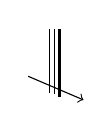
\begin{tikzpicture}[x=.6cm,y=.6cm]
\draw (0,1.5)--(0,.15); \draw (.10,1.5)--(.10,.12); \draw[line width=1pt] (.22,1.5)--(.22,.06);
\draw[->] (-.45,.50)--(.72,0);
\end{tikzpicture}}
\uline{Cont} \uuline{1} La relation ``$X\leq Y$'' ($\Longleftrightarrow X\ll Y$ et $X$ comp. $Y$) est une relation d'ordre
% @m1
% slanted
\margin{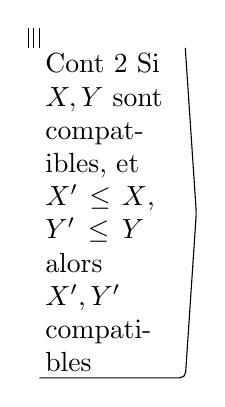
\begin{tikzpicture}
\node[inner sep=2pt,text width=1.7cm,align=left] (m34) {\uline{Cont} 2 Si $X,Y$ sont compatibles, et $X'\leq X$, $Y'\leq Y$ alors $X',Y'$ compatibles};
\draw (m34.north west)--++(0,.25); \draw ([xshift=-.07cm]m34.north west)--++(0,.25); \draw ([xshift=-.14cm]m34.north west)--++(0,.25);
\draw[rounded corners=2pt] (m34.north east)--([xshift=.14cm]m34.east)--(m34.south east)--(m34.south west);
\end{tikzpicture}}
% @fig2

\deleted{Cont 2} \inserted{\textcircled{\scriptsize Fig 2}} \deleted{Toute} Si $F\in\mathcal F$, deux éléments \inserted{$X,Y$} de $F$ sont compatibles, et $F$ est une partie \uline{fermée} de l'ens $M(\unsure{\leq|\ll})$.
% @fig3

\deleted{\unsure{Cont 3|Cont 4}} \inserted{\textcircled{\scriptsize Fig 3}} Si $F$ \deleted{et $G$ sont deux} \inserted{est une} figure, tt partie $F'$ de $F$ qui est fermée, est une figure (appelée \uuline{sous-figure}).
% @m2
% slanted
\margin{\uline{NB} Si \deleted{\unsure{$F,G$}} $F',F$ sont des figures telles que $F'\subset F$, alors $F'$ est fermée dans $F$, à cause de Fig 1}
% @empty
% The text enclosed by the long contour is also the conclusion of the lower Cor.
\figure{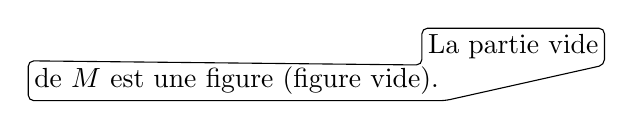
\begin{tikzpicture}[remember picture]
\node[anchor=south west,inner sep=2pt] (emptystart) at (5.0,.20) {La partie vide};
\node[anchor=west,inner sep=2pt] (emptyrest) at (0,0) {de $M$ est une figure (\uuline{figure vide}).};
\draw[rounded corners=2pt] (emptyrest.west) -- (emptyrest.north west) -- (emptystart.south west) -- (emptystart.north west) -- (emptystart.north east) -- (emptystart.south east) -- (emptyrest.south east) -- (emptyrest.south west) -- cycle;
\end{tikzpicture}}
% @fig1

\deleted{\unsure{Cont 3|Cont 4}} \inserted{\textcircled{\scriptsize Fig 1}} Si $X\in M$, l'ens \inserted{$F_{X}=M_{\leq X}$} des $Y\in X$ \deleted{tels} \deleted{\unsure{que}} que \unsure{$Y\leq X$} est une figure, qu'on appelle la ``\uuline{figure élémentaire}'' \unsure{définie} par \uline{la} multiplicité $X$.
% @cor

\uline{Cor}. \inserted{(de Cont 2 et Cont 4)} Si $M\neq\varnothing$, \tikz[remember picture,baseline]{\coordinate (corend) at (0,.15); \draw[overlay,->] (emptyrest.west) .. controls +(-1.2,-1.6) and +(-.4,-.8) .. (corend);}
% @nb

\uline{NB} Si $M=\varnothing$, \deleted{Si $M=\varnothing$} l'axiome \uline{Fig \unsure{3|4}} devient vide -- on le remplace par \unsure{:} \deleted{la partie} \deleted{la \unsure{partie vide de|partie vide est} $M$} la seule partie de $M$ (savoir la partie vide) est une figure.
% @cancelled

\deleted{\uline{Cor} (de \uline{Fig 1} et \deleted{\unsure{la}} \uline{Fig 2}) Si \deleted{$X$}, $Y,Z$ sont tels que \unsure{$Y,Z$}$\ll X$, et si $Y,Z$ st comp. à $X$, alors sont entre \unsure{eux}}

\scanpage{35}\mspage{34}
% @old
\deleted{\uline{Contrée finitiste} celle où toute figure}
% @fig

\deleted{\uline{Cont 5}} \inserted{\textcircled{\scriptsize Fig 4}} Soient $F$ et $\unsure{G|C}$ deux figures, telles que pour tt \deleted{$\forall$}$X\in F$, $Y\in G$, $x$ et $Y$ comp.
% @side
% slanted
\margin{On dit alors que $F$ et $G$ sont des \uline{figures compatibles}}
% @union
Alors $F\cup G$ est une figure -- \deleted{\unsure{tels|tel}} (\uuline{figure réunion}).
% @meet

Bien sur $F\cap G$ est une sous-figure commune de $F$ et de $G$.
% @oldcor

\deleted{Corollaire (de Fig 1, Fig 2, Fig 4 -- renforce le cor. précédent) Si $X,Y,\unsure{x'|X'},\unsure{y'|Y'}$ sont tels que $X'\ll X$, $Y'\ll Y$, et $\{X,Y\}$, $\{X',X\}$, $\{Y',Y\}$ comp., alors $X',Y'$ comp.}
% @fin

\uline{Contrée finitiste} Ou les figures sont finies. \deleted{Multistructure finitiste. \unsure{/}} \deleted{Une}
% @cor

\uline{Corollaire} \inserted{(de \uline{Cont} 2, \uline{Cont} 3, \uline{Cont} 5)} Les figures finies \deleted{sont} exactement les parties \uline{finies} de $M$, fermées pour $\leq$, formées d'é\deleted{\unsure{éléments|léments}} \deleted{\unsure{une}} d'é\deleted{\unsure{éléments|léments}} \inserted{\unsure{multisttes|multistés}} qui sont mutuellement compatibles.
% @donc

\unsure{Donc}, \deleted{la structure Contrée finitiste} \deleted{\unsure{une}} \inserted{les figures finies} \unsure{se pvt|se pt} \deleted{\unsure{et co}} connaître quand on connaît seulement $\ll,\unsure{\mathcal R|\mathcal Q}_{M}$. \inserted{Donc une contrée finitiste est connue, par les seules structures $\ll,\mathcal R_{M}$ ;}
% @question
Si on se donne deux telles relations, \inserted{(ordre, et rel. sym. réfle.)} satisfaisant \uline{Cont} 1, à quelles conditions les parties finies $\leq$-fermées \deleted{\unsure{que}} et formées d'éléments mut. compatibles (i.e les \uline{configurations}) satisf\deleted{\unsure{ass|ais}}ont-elles \uline{Cont} 2 à \uline{Cont} 5, ?

\scanpage{36}\mspage{35}
% @opening
\deleted{\unsure{Il faut que|figure} \unsure{l'on a|On a}} La condition est la suivante ; \deleted{\unsure{qu'on requiert}}
% @fini

\uline{Cont} \deleted{\unsure{4|2|3}}$3'$ (Facultative dans le cas non finitiste) \deleted{$\forall$} Pour tout $X\in M$, \deleted{la figure} \inserted{l'ens} $M_{\leq X}$ est fini. (i.e. les figures élémentaires sont finies)
% @dims

Par contre, on exige en tous cas que la \uuline{dimension combinatoire} de tout \deleted{\uline{Cont} 3 La} $X\in M$ soit finie (i.e. $\dim\text{ comb }M_{\leq X}$ finie), et plus \deleted{géné} précisément encore
% @mark
% slanted
\margin{\uuline{\unsure{devant|demain}}\hspace{2pt}\tikz[baseline]{\draw (0,-.2)--(0,.4) (.045,-.2)--(.045,.4) (.09,-.2)--(.09,.4);}}
% @sup
\[
\uline{\text{Cont}}\,3 \quad \text{Si } X\in M,\qquad
\underbrace{\mathop{\mathrm{Sup}}\limits_{X'\ll X}\,\mathrm{dim\,comb}\,M_{\leq X}}_{\text{\uline{dimension} (géom) de }X}<\infty
\]
% @place
On appelle \uuline{lieu} un \unsure{élémt|élément} de $M$ minimal pour $\ll$. On dénote par $\mathcal L$
% @subset
\[
\mathcal L\subset M
\]
% @endplace
l'ens des lieux.
% @shadow

Pour tout $X$, son \uuline{ombre} \inserted{(fermée)} sur $\mathcal L$ est l'ens $\mathcal L_{X}$ des lieux $x$ \deleted{$\unsure{\ll X}$} ``de $X$'' i.e. tels que $x\ll X$. On pose
% @sidelf
% slanted
\margin{$\mathcal L_F=\bigcup_{X\in F}\mathcal L_X$ s'appelle \uline{l'ombre de} \uline{la} figure \uline{$F$}}
% @lf
\[
\mathcal L_X^{\circ}=\mathcal L_X\setminus\bigcup_{Y<X}\mathcal L_Y
\]
% @axiom

\uline{Cont} \deleted{5}4 \quad a) $\forall X\in M$, on a $\mathcal L_X^{\circ}\neq\varnothing$

% @axiomb
b) Si $X,Y$ sont compatibles et distincts on a
% @disjoint
\[
\mathcal L_X^{\circ}\cap \mathcal L_Y^{\circ}=\varnothing
\]

\scanpage{37}\mspage{36}
% @schol
\uline{Scholie} \deleted{L'applicat\unsure{ion|.}} Soit $\unsure{F|\mathcal F}$ une figure. Alors

% @maponelead
a) L'application
% @mapone
\diagram{\begin{tikzcd}[ampersand replacement=\&,column sep=small]
X\arrow[r,mapsto] \& \mathcal L_X=\widetilde X \& F\arrow[r,phantom,"{\relbar\joinrel\relbar\!\shortmid}" description] \& \mathcal P(\mathcal L)
\end{tikzcd}}
% @image
est injective, et son image \inserted{$\widetilde F$} est un ensemble de parties ``admissible'' de l'ensemble $\mathcal L$, i.e.
% @unions
\[
\text{a)}\quad\forall\widetilde X,\widetilde Y\in\widetilde F,\quad\text{on a}\quad
\widetilde X\cap\widetilde Y=\bigcup_{\substack{\widetilde Z\in\widetilde F\\ \widetilde Z\subset\widetilde X\cap\widetilde Y}}\widetilde Z
\]
% @partb
\[
\begin{aligned}
&\text{b)}\quad \forall\widetilde X\in\widetilde F,\quad\text{posant}\quad
\partial\widetilde X=\bigcup_{\substack{\widetilde Y\in\widetilde F\\ \deleted{\unsure{X|Y}}\widetilde Y\subsetneq\widetilde X}}\widetilde Y,\quad\text{et}\\
&\qquad\widetilde X^{\circ}=\widetilde X\setminus\partial\widetilde X,\quad\text{on a}\qquad\qquad \widetilde X^\circ\neq\varnothing
\end{aligned}
\]
% @margin
% slanted
\margin{\uline{\unsure{Déf}} La figure $\partial X=\{Y\in M\mid Y<X\}$ s'appelle \uline{le bord} de $X$}
% @name

On \deleted{b) L'application $X$} \inserted{appelle} $\widetilde X^\circ$ l'\uline{ombre ouverte} de $\widetilde X$ sur $\mathcal L$, $\partial\widetilde X$ \deleted{\uline{l'ombre \unsure{frontière|fr.}}} \inserted{\uuline{bord d'ombre}}
% @maptwolead

b) L'application
% @maptwo
\diagram{\begin{tikzcd}[ampersand replacement=\&,column sep=small]
X\arrow[r,phantom,"{\unsure{\longmapsto|\mapstochar\relbar\joinrel\relbar}}" description] \& \mathcal L_X^\circ=\widetilde X^\circ \& F\arrow[r,phantom,"{\longrightarrow}" description] \& \mathcal P(\mathcal L).
\end{tikzcd}}
% @partition
est injective, et \deleted{les de $F$} les images forment une \uline{partition} de l'ombre $\mathcal L_F$ de la figure $F$, indexée par $F$.
% @order

c) \deleted{Soit} La relation $\leq$ sur $F$ est celle induite par la relation d'inclusion sur les ombres. Si $X,Y\in F$, alors conditions équiv.
% @four
\[
\left\{\begin{aligned}
&\text{(i)}\;X\leq Y\\
&\text{(ii)}\;\widetilde X\unsure{\subseteq|\subset|\in}\widetilde Y\\
&\text{(\unsure{iii})}\;\widetilde X^\circ\unsure{\subseteq|\subset|\in}\widetilde Y\\
&\text{(iv)}\;\widetilde X^\circ\cap\widetilde Y\neq\varnothing
\end{aligned}\right.
\]

\scanpage{38}\mspage{37}
% @d
d) \deleted{Les} Pour tt sous figure $\unsure{F'|\mathcal F'}$ de $F$, on a \deleted{$\mathcal L_F$} $\widetilde F'=\mathcal L_F\subset \mathcal L$ son ombre, et
% @map
\diagram{\begin{tikzcd}[ampersand replacement=\&]
\unsure{\mathbb F'|F'}\arrow[r] \& \widetilde F'
\end{tikzcd}}
% @bijection
est une bijection de l'ens des sous-figures de $F$, avec l'ens des parties de $\widetilde F$ (ombre de $F$) qui sont ``fermées'' pour le rec. admissible de $\widetilde F$ par \inserted{l'ens.} des $\widetilde X$ ($X\in F$).
% @prop

\uline{Proposition} Soit $M$ une contrée, $M'$ une sous contrée, \deleted{\unsure{on prend|on pourrait}} i.e. une partie de $M$, fermée pour $\ll$, et munie des relations $\underset{M'}{\ll},\unsure{\mathcal R|\mathcal Q}_{M'}$ induites par $M$, et de l'ens \inserted{$\mathcal F_{M'}$} des parties \deleted{$M'$} \inserted{de $M'$} qui sont des figures de $M$. Alors
% @triple
\[
(M',\underset{M'}{\ll},\mathcal F_{M'})
\]
% @conds
satisfait les conditions \uline{Cont} 1 : \uline{Cont} 4, et si $X\in M'$, ses \unsure{dimens|dimm's} combinatoires et géométrique sont les \unsure{$=$s|$\Rightarrow$} dans $M$ et dans $M'$, Si $\mathcal L'=M'\cap \mathcal L$, alors pour \deleted{tout} $\mathbb F\in\mathcal F_{M'}$, son ombre \inserted{(fermée)} pour $M$ ou $M'$ est la $=$, si si $X\in M'$, \deleted{$X$} son ombre ouverte est la $=$ \inserted{pour $M$ et pour $M'$}, D $=$ pour le bord $\partial X$. Les conditions Fig 1 : Fig 4 sont valables dans $M'$. La condition \uline{Cont} $3'$ \deleted{\unsure{est valable}} \inserted{\unsure{est}}

\scanpage{39}\mspage{38}
% @continuation
également stable par passage à une sous-contrée. Enfin, si $\unsure{C|\mathcal C}$ est finitiste, $\unsure{C'|C}$ aussi\unsure{?|:|.}
% @disj

\uuline{\deleted{Figures} disjointes} On dit que deux figures sont disjointes si elles sont compatibles, et si leur intersection est vide (\unsure{pas|que} de multistrates communes).
% @warn
% slanted
\margin{\uline{attention} Pour que deux figures ($=$ élémentaires) soient disjointes, il \unsure{est} \uuline{néc}, mais \deleted{\unsure{pas}} \inserted{néc} \unsure{suffis|suffisant} que leurs ombres soient disjointes (\unsure{c.à.d.} : \unsure{cp paires|cp pour} \unsure{simplifient} pour deux lieux !)}
% @warn2
\margin{\unsure{si|Si} \deleted{\unsure{de}} elles sont compatibles, \deleted{\unsure{et}} et \unsure{?}\par
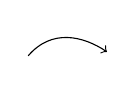
\begin{tikzpicture}[x=1cm,y=1cm]\draw[->] (0,0) .. controls (.3,.35) and (.7,.25) .. (1,.05);\end{tikzpicture}}
% @objects
On dit que \inserted{\uline{deux multistrates}} $X,Y$ sont \uline{disjointes} si $F_X,F_Y$ le sont, \inserted{i.e. s'il n'existe pas de \deleted{\unsure{$X$}\illegible{2}} $Z\in M$, avec $Z\leq X,Y$}
% @equiv
% slanted
\margin{ou ce qui revient au $=$, si elles sont comp. et \deleted{l'intersection} \deleted{de leurs} ombres sont disjointes (\unsure{ensemblmt|ensemblistmt})}
\margin{\begin{tikzpicture}[x=1cm,y=1cm]\draw (0,0) .. controls (1.4,.1) and (1.6,1.7) .. (1.3,2.4) .. controls (1.1,2.9) and (.3,3) .. (.05,2.75);\end{tikzpicture}}
% @all
% slanted
\margin{Pour que $F,G$ soient disj., il f et s. que $\forall X\in F$, $Y\in G$, $X$ et $Y$ soient disj.}
\margin{\begin{tikzpicture}[x=1cm,y=1cm]\draw (1.3,3.2) .. controls (.7,3.15) and (.6,2.6) .. (.8,2.25) .. controls (1.05,1.7) and (1,1) .. (1,0);\end{tikzpicture}}
% @refine

\deleted{Soit de} \deleted{deux} figures $F,G$, on dit que $F$ \uuline{raffine} $G$ (et on écrit $F\ll G$) si $\forall X\in F,\ \exists Y\in G$ tel que $X\ll Y$. Pour deux figures élémentaires $F_X,F_Y$ cela signifie donc \unsure{simplemt|simplmt} que $X\ll Y$.
% @prop

\deleted{Si $F$ raffine $G$} \uline{Proposition} Pour que $F$ soit une sous-figure de $G$, il f et s. que $F$ raffine $G$, et soit compatible à $G$
\margin{\begin{tikzpicture}[x=1cm,y=1cm]\draw (0,0)--(0,1.15);\end{tikzpicture}}
% @proof

$\Longrightarrow$ trivial, pour prouver $\Longrightarrow$ on note que \inserted{ds la déf. du raffinement,} $X\ll Y$ \deleted{et} $X$ comp. à $Y$ \deleted{\unsure{et}} implique $X\leq Y$, donc $X\in G$ à cause de Fig 2.

\scanpage{40}\mspage{39}
% @axiom
\uline{Cont} 5 Soient $X.Y\in M$, $X$ et $Y$ \uline{disjoints}. Alors pour $X'\ll X$ et $Y'\ll Y$, $X'$ et $Y'$ sont \deleted{disjoints} \deleted{compatibles} disjoints
\margin{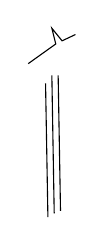
\begin{tikzpicture}[x=1cm,y=1cm]\draw (0,0)--(-.03,1.7) (.08,.05)--(.05,1.8) (.16,.08)--(.13,1.8);\draw (-.25,1.95)--(.1,2.2)--(.05,2.4)--(.18,2.24)--(.35,2.32);\end{tikzpicture}}
% @sim
% slanted
\margin{S'apparente à \uline{Cont} 2 (page 33)}
% @cancelone

\figure{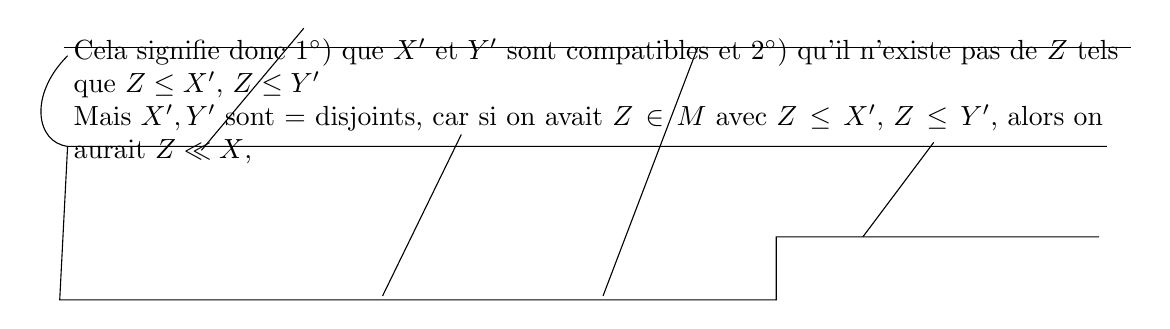
\begin{tikzpicture}[x=1cm,y=1cm]
\node[anchor=north west,inner sep=2pt,text width=13.5cm] (cancelled) at (0,0) {\deleted{Cela signifie donc $1^\circ$) que $X'$ et $Y'$ sont compatibles et $2^\circ$) qu'il n'existe pas de $Z$ tels que $Z\leq X'$, $Z\leq Y'$}
% @canceltwo

\deleted{Mais $X',Y'$ sont $=$ disjoints, car si on avait \inserted{$Z\in M$ avec} $Z\leq X'$, $Z\leq Y'$, alors on aurait $Z\ll X$,}};
\draw (-.05,-.2)--(13.5,-.2);
\draw (0,-.3) .. controls (-.5,-.8) and (-.4,-1.4) .. (0,-1.45)--(13.2,-1.45);
\draw (0,-1.45)--(-.1,-3.4)--(9,-3.4)--(9,-2.6)--(13.1,-2.6);
\draw (3,.05)--(1.7,-1.5) (5,-1.3)--(4,-3.35) (8,-.2)--(6.8,-3.35) (11,-1.4)--(10.1,-2.6);
\end{tikzpicture}}
% @split

Se décompose en deux

% @splita
\textcircled{\scriptsize a} Sous les condition de Cont 5, $X'$ et $Y'$ st \uline{compatibles}
% @noz

\textcircled{\scriptsize b} \deleted{Si $Z$} $\nexists\ Z\in M$ avec $Z\ll X$, $Z\ll\deleted{X}Y$.
% @ip

(i.e si $X,Y$ compatibles, alors $M_{\leq\unsure{x|X}}\cap M_{\leq Y}=\varnothing$ implique même $M_{\ll X}\cap M_{\ll Y}=\varnothing$)
% @cor

\uline{Cor} Si $\unsure{F|\mathcal F}$ et $\unsure{G|\mathcal G|\mathbb G}$ sont des figures disjointes, alors pour tt raffinement $F'$ de $F$ et tt raffinement $G'$ de $G$, $F'$ et $G'$ sont disjointes.
% @addcor
% slanted
\margin{\uline{Cor} Pour que deux figures \deleted{\unsure{$F,G$}} $F,G$ soient disjointes, il f et s q. pour tous $x\in\widetilde F,y\in\widetilde G$, q $x$ et $y$ disjoints}
% @remark

\uline{Remarque} Soit $M'$ une sous-contrée. Pour deux figures $F,G$ de $M'$, \deleted{leur} \inserted{ou deux \unsure{multi-formes|multi-strates} $X.Y$} dire qu'elles sont disjointes au sens de $M'$ ou de $M$ est pareil, et de $=$ pour la notion que $F$ raffine $G$ Si $M$ satisfait \uline{Cont} 5, $M'$ aussi. \inserted{it\deleted{\unsure{ou|em}} pour \uline{Cont} 6 qui suit}
\margin{\begin{tikzpicture}[x=1cm,y=1cm]\draw (0,.6) .. controls (-.2,.2) and (.2,.1) .. (1.1,.1) .. controls (1.6,.1) and (1.5,-.2) .. (1.65,-.5)--(1.9,-.2);\end{tikzpicture}}
% @six

\uline{Cont 6} (Facultatif ?) Si $X$ et, $Y\in M$ sont tels que \deleted{$\forall$} $\widetilde X\cap\widetilde Y=\varnothing$ \uuline{et} tout $a\in\widetilde X$ est comp. à \deleted{\unsure{tout|tous}} $y\in\widetilde Y$, alors $X$ et $Y$ sont disjoints
% @foot
\margin{\tikz[baseline]{\draw[<->] (0,.68)--(.52,.20); \draw (.58,-.13)--(.58,.30) (.63,-.13)--(.63,.30) (.68,-.13)--(.68,.30); \draw (-.08,-.05) ellipse (.035 and .06); \draw (-.08,-.05)--(-.05,.26);}\,\unsure{avec|donc} tt elt $\unsure{\bar X|\widetilde X|x}$ disjoint de tout $y\in\widetilde Y$}

\scanpage{41}\mspage{40}
% @title
\uline{Contrées induites}

% @ind
$1^\circ$) Soit $F$ une figure. Contrée \inserted{induite} $C_F$, \deleted{définie par les} c'est la partie fermée de $M_{\ll}$ engendrée par $F$, i.e. l'ens des $X^{\deleted{\unsure{F|f}}}\in M$ tels que $X$ raffine $F$.
% @lieu
% slanted
\margin{\uline{NB} L'ens des lieux de la contrée $C_F$ n'est autre que l'ombre de $F$}

% @resid
\uline{Contrée résiduelle} C'est la \inserted{sous} contrée $C_{\complement F}$ \deleted{\unsure{form|for}} formée des $X$ \inserted{$\in M$} qui sont disjoints de $F$. Par C\deleted{\unsure{o|on}}onst. 5, elle est \deleted{stable} \deleted{pour} fermée dans $M^{\unsure{\deleted{\leq}|\deleted{z}|\sharp}}_{\ll}$.
% @lieures
% slanted
\margin{\deleted{\unsure{Le|La}} L'ens des lieux de $C_{\complement F}$ est contenu dans $\complement_{\mathcal L}\widetilde F$, mais ne lui est \deleted{\unsure{égal|néces|pas}} pas \unsure{néc\textsuperscript{t}|néc\textsuperscript{t}.} égal.}

% @fig
\deleted{Cor} Soi\deleted{ent}t $F$ une figure, $G$ une \deleted{\uline{Subdivision}} sous figure. La contrée résiduelle de $F$ dans $G$ est par définition
% @meet
\[
 C_{\deleted{G}F}\cap C_{\complement\deleted{F}G}
\]

% @sub
\uline{Subdivision} Soit $F$ \inserted{$\subset M$} une figure, \deleted{et} On appelle \uline{subdivision} de $F$ une figure\unsure{\textsuperscript{o}|.} $F'\subset M$ telle que
% @a

a) $F'$ soit un raffinement de $F$
% @b

b) $F'$ soit maximale \inserted{pour $\subset$}, parmi les \deleted{raffi} figures qui raffinent $F$.
% @nb

\uline{NB} Si $F'$ raffine $F$, alors son ombre $\widetilde F'$ est contenue dans celle $\widetilde F$ de $F$.

\scanpage{42}\mspage{41}
\uline{Prop} Soit $F'$ un raffinement de $F$. Conditions équivalentes

a) $F'$ est une subdivision

b) Il n'existe pas de $X\in M$ qui raffine $F$, et disjoint de $F'$

c) \deleted{Il n'existe pas \unsure{Ou bien} $\widetilde F'=\widetilde F$, sinon, \illegible{1} \unsure{de} \unsure{il} il n'existe pas de lieu du $F$} Il n'existe pas de lieu dans l'ombre $\widetilde F$, qui soit disjoint de $F'$ i.e. \inserted{(\deleted{par}\unsure{Cont|Cond|Corol} 6)} $\forall\deleted{\unsure{x}}x\unsure{\in|+}\widetilde F\setminus\widetilde F'$, $\exists\,y\in\widetilde F'$ tel que $x$ et $y$ \uline{non compatibles}, ou (positivement) : Si $x\in\widetilde F$ est compatible à tout élément de $\widetilde F'$, il est dans $\widetilde F'$.

\uline{Dém} $a\Longrightarrow b$, car si $X\in M$ raffine $F$ et est disjoint de $F'$, alors la figure $F\cup F_X$ est un raffinement de $F$, \unsure{strictmt|strictement} plus grand que $F'$,

$b)\Longrightarrow c)$ tautologique

$c)\Longrightarrow a)$ Si on avait, $F'\unsure{\subset|\in} \uline{F''}\not\ll F$, soit $X\in F''$, tel que $X\notin F'$, et soit $x\in\widetilde X^\circ$. Alors $x\in\widetilde F\setminus\widetilde F'$, et \deleted{je dis} que $x$ est compatible à $F'$ donc c) n'est pas vérifié.
% slanted
\margin{à vérifier}
\figure{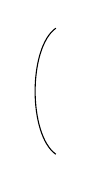
\begin{tikzpicture}[x=1cm,y=1cm]\draw (0.25,0.8) .. controls (-0.1,0.55) and (-0.1,-0.55) .. (0.25,-0.8);\end{tikzpicture}}

Mais on a utilisé que $x$ est compatible à $F'$, il faut un axiome pour l'assurer.

\uline{Cont} 7 Soient $X,\deleted{\unsure{X}}Y\in M$, \inserted{$X$ et $Y$ compatibles} $X\ne Y$. \inserted{(donc $\widetilde{\deleted{\unsure{Y}}X}^\circ\cap\widetilde Y^\circ=\varnothing$)} Alors tout $x\in\widetilde X^\circ$ est disjoint de tout $y\in\widetilde Y^\circ$ (ou, ce qui revient au $=$ par Cont 6, \deleted{tout} $x\in X^\circ$ est disjoint de $Y$)
\figure{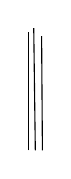
\begin{tikzpicture}[x=1cm,y=1cm]\draw (0,0)--(0,1.5);\draw (0.09,0)--(0.07,1.55);\draw (0.18,0)--(0.17,1.45);\end{tikzpicture}}

\uline{Cor. 1} Soient $F$ une figure, $F'$ une sous-figure et $X\in F\setminus F'$. Alors $\forall\,x\in X^\circ$ est \deleted{compatible} \inserted{disjoint} de $F'$.

\scanpage{43}\mspage{42}
\uline{Cor. 2} Soit $F$ une figure. Deux lieux dans \deleted{\uline{Cor. 2} Soit $F$ une figure. Deux} l'ombre de $F$, qui appartiennent à des ombres ouvertes de strates distinctes, sont \uline{disjoints}.

Soient $\deleted{X}F$ une figure, \deleted{$X\in M$ un raffinement de $F$,} \inserted{$F'$ un raffinement} de $F$. Je \unsure{veux|vaux} definir une application
\[
 F'\longrightarrow F
\]
en associant : tt $X'\in F'$ \{l'unique\} $X\in F$ tel que
\[
 \widetilde{X'}^\circ\subset\widetilde X^\circ
\]
(ou encore le \uline{plus petit} \deleted{\unsure{des|x|X}} $X'\in F$ tel que $\widetilde{X'}^\circ\subset\widetilde X$). Savons-nous déjà qu'un tel $X$ existe, i.e. que \unsure{la|R} relation d'équiv. canonique sur l'ombre de $F'$, est plus fine que celle induite par l'ombre de $F$ ? Soit $X$ un élément de $F$ \uline{minimal}, parmi ceux satisfaisant $X'\ll X$ (existe, à cause de l'axiome de dim), savons nous que dès lors $\widetilde{X'}^\circ\subset\widetilde X^\circ$ ? \deleted{Soit} On sait que $\widetilde{X'}\subset\widetilde X$ donc si $x\in X'^\circ\inserted{\subset\widetilde{X'}}$, on a $x\in\widetilde{\deleted{\unsure{X|Y}}Y}^\circ\subset\widetilde Y$ pour $Y\leq X$, on veut prouver que $Y=X$. Il semblerait qu'il manque quelque chose.

\scanpage{44}\mspage{43}
\uline{Cont 8} Soit $X,Y,X'$ dans $M$, $Y\ll X$, $X'<X$. Considérons l'ens des $Y'\in\deleted{ M}F_Y$ (i.e. $Y'\leq Y$) tels que $Y'\ll X$ :
% slanted
\margin{Axiome du raffinement induit.}
\diagram{\begin{tikzcd}[ampersand replacement=\&,row sep=0.1em,column sep=0.35em]
Y \& \ll \& X\\
\tikz[baseline=-.5ex]\node[rotate=90,inner sep=0pt] {$\leq$}; \& {} \& \tikz[baseline=-.5ex]\node[rotate=90,inner sep=0pt] {$\unsure{<|\leq}$};\\
Y' \& \ll \& X'
\end{tikzcd}}

(lesquels forment une sous-figure $R_{X'}$ de le multistrate $\deleted{\unsure{F|\in}}F_Y$, \deleted{qu'on appellera} raffinant $X'$, et qu'on appellera le raffinement de $X'$, induit par $Y$ sur $X'$). Alors \unsure{tout\deleted{e}|toute} raffinement commun $Z$ de $Y$ et de $X'$ raffine un des $Y'$, i.e. raffine $R_{X'}$. (Donc Tout figure qui raffine à la fois $\deleted{\unsure{Y|F}}F_Y$, et $F_{X'}$, raffine $R_{X'}$, qui est \deleted{\unsure{donc} la borne} borne inf. de $F_Y$ et $F_{X'}$ pour la relation $\ll$) En particulier,
\[
 :\quad \widetilde Y\cap\widetilde{X'}=\bigcup_{Y'\in R_{X'}}\widetilde{Y'}
\]

\uline{Cor} \deleted{\unsure{Soit} $x\in\widetilde{\unsure{Y|X}}^\circ$,} Supposons que $\deleted{\unsure{\exists}}\nexists\,X_1\in M$, avec $Y\ll X_1<X$ (c'est la situation de tantôt) Alors $\widetilde Y^\circ\subset\widetilde X^\circ$.

En effet, si $x\in\widetilde Y^\circ$, \unsure{si on|s'on} avait $x\in\widetilde{X'}$ pour $X'<X$, on aurait $x\in\widetilde{Y'}$ avec $Y'\in R_{X'}$, donc $Y'\Rightarrow\deleted{\unsure{X}}Y$ par déf. de $\widetilde Y^\circ$, donc $Y\ll X'_{\deleted{\unsure{1}}}<X$, \inserted{contraire à hyp.}

\scanpage{45}\mspage{44}
\uline{Corollaire} Si $\deleted{\unsure{X}}Y\ll X$, alors \deleted{la relation} toute ombre ouverte d'une \deleted{\unsure{figure|strate de}} \inserted{strate eff.} $Y$ est contenue dans l'ombre ouverte d'une strate de $X$. Plus généralement et par suite, pour tte figure $F$ et \deleted{\unsure{t}} \deleted{sous-figure} \inserted{raffinement} $F'$ de $F$, toute \deleted{strate} \deleted{de ombre ouverte d'une} strate ouverte de $F'$ est contenue dans une (unique) strate ouverte de $F$.

\deleted{\uline{\unsure{Cont|Cond}}. 8 Si \unsure{/}}\enspace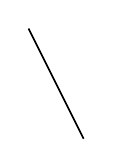
\begin{tikzpicture}[baseline=0pt]\draw[line width=.6pt] (0,.4)--(.7,-1);\end{tikzpicture}

Je viens de m'apercevoir que dans le cas du pseudo disque, \deleted{une} deux lieux disjoints \deleted{\unsure{cq}} \inserted{$x,y$} de l'intérieur (lesquels définissent donc deux ``raffinements'' dudit pseudo-disque), qu'il existe une ``Subdivision'' du disque dont ils soient des \unsure{noeuds|nœuds}. [\uline{NB}. Les \uline{noeuds} d'une figure \inserted{$\deleted{F}F$} sont les multistrates \inserted{de $\deleted{\unsure{X|F}}F$} réduites à un lieu, i.e. les éléments de $F\cap\mathcal L$] Donc \deleted{\unsure{la no}} il n'y a pas lieu de considérer $\{x,y\}$ comme un ``raffinement'', vu qu'il ne s'étend pas en une subdivision. Donc il est inapproprié

\scanpage{46}\mspage{45}
de définir une figure $F'$ comme un \uline{\unsure{raffinant|raffinement}} de $F$, si chaque $X'\in F'$ \deleted{\unsure{déf}} est un raffinement d'un $X\in F$. Donc il vaut mieux prendre comme notion primitive celle de \uline{subdivision} d'une \deleted{\unsure{mul}} \inserted{figure}, (qui va se ramener ; celle d'une multistrate), et définir un raffinement d'une figure comme sous-figure d'une subdivision.

Donc, nouveau départ !

Une contrée $C$ est définie par un triple
\[
 (M,\mathcal F,\Sigma)
\]
où $ M$ est un ens (ens. des \uline{multistrates}), $\mathcal F$ un ensemble de parties de $ M$ ($\mathcal F\in\mathcal P(\mathcal P(M))$), \inserted{\unsure{appelées|appelés} \uline{figures},} et $\Sigma$ une relation sur $\mathcal F$ dite : $F'$ \uline{subdivise} $F$. \unsure{Axiomes|Axiome}
% slanted
\margin{Si $F\in\mathcal F$, les $X\in F$ sont les (multi)strates de $F$}

\uline{C 1} Pour tout $X\in M$, $\exists$ \unsure{une|un} plus petite \deleted{partie} figure \deleted{qui} $F_X\unsure{\subset|{,}}$ telle que $X\in F$.

On l'appelle la \uline{figure élémentaire} définie par $X$. On écrit
\[
 X\leq Y\ \overset{\mathrm{def}}{\Longleftrightarrow}\ F_X\subset F_Y\qquad\text{i.e. }X\in F_Y
\]
et on trouve une relation d'\uline{ordre}$^{*}$ $\leq$ sur $ M$.\textsuperscript{$*$}
\margin{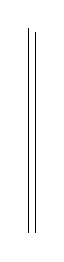
\begin{tikzpicture}\draw (0,0)--(0,2.6);\draw (.09,0)--(.09,2.55);\end{tikzpicture}}
% slanted
\margin{$^{*}$ On veut que ce soit une relation d'ordre et pas seulement de préordre, i.e. \uline{C$'$1} si \deleted{\unsure{pr}} $X\ne Y$, $\exists$ $F\in\mathcal F$ qui \unsure{contient} un des deux \unsure{ms} $X,Y$, et pas l'autre, i.e. $F_X\ne F_Y$.}
% slanted
\margin{-- i.e. $\mathcal F$ \unsure{séparé|sépare} les éléments de $ M$}

\scanpage{47}\mspage{46}
% slanted
\margin{Ainsi, $M$ s'identifie à un ens de parties de $\mathcal F$ (savoir les $F_X$) i.e. à l'ens des figures élémentaires. \deleted{Donc on peut considérer que la structure est \unsure{portée} par $\mathcal F$, muni de $\mathcal F_{\unsure{\mathrm{él}|\mathrm{el}}}$ et de $\unsure{\Sigma}$, la relation de subdivision (relation d'ordre)} \deleted{Il y a une sorte de symétrie -- on travaille sur $\mathcal F$, \unsure{en tant|ou bien|comme} \inserted{\unsure{axiomatique des|par les axiomes des}} \unsure{et tantôt} sur $ M$,  1°) relation d'ordre $\unsure{C'|\leq}$ (subdivision, ou $\ll$ raffinement) et ens. de parties (élémentaires, les figures).}}
\deleted{Cela étant}

\deleted{$\unsure{X}\ll Y\quad\unsure{F'}\unsure{\supset|\subset}F_X$} Si $F$ est une figure, alors $X\in F_{\deleted{\unsure{X|x}}}$ équivaut : $F_X\subset F$, qui implique que pour tout $Y\in F_X$ \inserted{i.e. $Y\leq X$} on a $F_Y\subset F$ i.e. $Y\in F$. Ainsi, $F$ est une partie de $ M$ \uline{fermée} pour $\leq$.

On dit que deux figures \inserted{$F,G$} sont \uline{compatibles} si $F\cup G$ est une figure, et que $X,Y\in M$ sont \uline{compatibles} si $F_X,F_Y$ le sont

\uline{C \deleted{\unsure{2|3}}\unsure{3|2}} Pour que $F$ et $G$ soient compatibles, il f. et s. que $\forall\,\unsure{x|X}\in F,\ Y\in G$, $X$ et $Y$ le soient.
\margin{\tikz{\draw (0,0)--(0,.8);\draw (.06,0)--(.06,.8);}}
% slanted
\margin{correspond à Fig 4}

\uline{Cor} \deleted{En particulier si $X$} Pour que $X,Y\in M$ soient compatibles, il f et s. qu'ils \uuline{app}artiennent à une figure

\deleted{\uline{C 3} Si $F$ est.}
% slanted
\margin{\tikz[baseline=(a.base)]{\node[inner sep=1pt] (a) {intervertir}; \draw[->] (a.north) .. controls +(0,.6) and +(-.5,0) .. (1.4,1); \draw[->] (a.south) .. controls +(0,-.6) and +(-.5,0) .. (1.4,-1);}}

\uline{C \deleted{\unsure{3|2}}\unsure{2|3}} Soit $F$ une figure, alors tte partie de $F$ fermée pour $\leq$ est aussi une figure (i.e. pour qu'une partie $F'$ de $F$ soit une figure, il f et il \uline{suffit} qu'elle soit fermée pour $\leq$).
\margin{\tikz{\draw (0,0)--(0,.8);\draw (.06,0)--(.06,.8);}}

(\uline{Sous-figures}) Si $ M\ne\varnothing$ cela \deleted{\unsure{signifie}} implique que la partie vide de $ M$ est une figure. Si $ M=\varnothing$, \deleted{cela implique que} \inserted{on aura $\mathcal F=\varnothing$} \deleted{si $\mathcal F$} ou $\mathcal F=\{\varnothing\}$, et on suppose que c'est le deuxième cas : \uline{figure vide} existe tjrs
% slanted
\margin{\uline{Contrée vide} si $ M=\varnothing$}

\scanpage{48}\mspage{47}
\uline{Définition} Soient $F,\deleted{F'}G$ deux figures. On dit que $\deleted{F'}G$ est un \uline{raffinement} de $F$, s'il existe une \deleted{\unsure{raffinée|raffin}} subdivision $F'$ de $F$, telle que $G\subset F'$ \inserted{sous-figure}.
% slanted
\margin{On écrit $F\ll G$}
\figure{
\begin{tikzpicture}[x=1cm,y=1cm,scale=.8]
\fill (0,0) .. controls (.1,.2) and (.16,.2) .. (.19,.55) -- (.3,.65) -- (.5,.6) .. controls (.48,.3) and (.7,.25) .. (.45,-.15) -- (.34,-.2) -- (.37,.38) -- (.12,.44) -- cycle;
\fill (1.9,.15) -- (1.85,.3) -- (2.1,.35) -- (2.35,.35) -- (2.35,.5) -- (2.55,.3) -- (2.65,.63) -- (3.35,.65) -- (3.35,.55) -- (3.5,.53) -- (3.35,.45) -- (3.45,.35) -- (3.25,.18) -- (2.7,.1) -- cycle;
\foreach \x/\y in {.6/.55,.7/.4,.4/-.28,2.1/.05,2.3/.7,2.5/-.02,3.4/.02,3.3/-.08}{\fill (\x,\y) circle(.025);}
\end{tikzpicture}}

On veut que ce soit une relation d'ordre, et pour ceci on va poser

\uline{C 4} Soient $F$ une figure, $G$ une sous-figure \inserted{(i.e. $G$ figure et $G\unsure{\subset|\in}F$)}, $G'$ une subdivision de $G$. Alors \deleted{il existe une subdivision $F'$ de $F$,} \inserted{$G'\cup(F\setminus G)$ est une} subdivision \inserted{de $F$}, et la réunion est disjointe (i.e. \deleted{hors de $G$} \margin{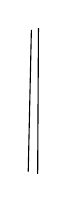
\begin{tikzpicture}[x=1cm,y=1cm]\draw (0,0)--(.04,1.8);\draw (.12,-.03)--(.13,1.82);\end{tikzpicture}}
\[
 \boxed{G'\cap F\subset G}
\]
\deleted{donc} $G'\cap F=G'\cap G$).
% slanted
\margin{C'est \unsure{démenti|évidemment} \unsure{par exemple} les strates fermées et str. augmentées\ldots\ \uline{cf plus} bas.}
% slanted
\margin{i.e \unsure{toute} multistrate d'une subdivision de $G$ qui est \uline{compatible} avec $F$ \uline{est dans $G$}. OK}
\margin{OK $\longrightarrow$}
\margin{Corriger : $\exists$ subdivision qui induit $G'$ $+$ la relation $G'\cap\unsure{F^{\to}\subset|F'\subset|F\subset}G$}

\uline{Cor. 1} \uline{Toute} \deleted{raffinement} \inserted{\uline{subdivision}} \uline{d'une sous figure de $F$ est induite par une ``subdivision de $F$}.
\margin{\begin{tikzpicture}\draw (.18,0) .. controls (-.15,.25) and (-.12,.85) .. (.1,1.2);\end{tikzpicture}}

\uline{Cor 2} La relation de raffinement entre figures
\[
 F\ll G
\]
est une relation d'ordre.
% slanted
\margin{OK.}

\deleted{\uline{\unsure{C 5}} \inserted{\uline{Proposition}} Soient $X,\deleted{\unsure{Y}}\in M$, \inserted{$\deleted{F}G\in\mathcal F$.} Pour que $X\in\deleted{\unsure{F_Y}}G$ \deleted{i.e. $F_X\subset F_Y$} il f. et s. que $X$ et $\deleted{\unsure{Y}}G$ compatibles (i.e. $F\equiv F_X\cup\deleted{\unsure{F_Y}}G$ une figure) et $X$ \deleted{raffine} $\inserted{\ll}\deleted{\unsure{F_Y}}G$ i.e $F_X$ raffine $\deleted{\unsure{F_Y}}G$.}
% slanted
\margin{C'est la \deleted{Condition} \inserted{définition} de $\leq$ via $\ll$ et $R$}

\deleted{\deleted{\unsure{On}} Supposons en effet que $X$ et $F$ compatibles \deleted{il \unsure{faut} $X\unsure{\text{et}|,|\in}Y\in F$}, $F$ figure, et que $F_X$ raffine la sous-figure $F_Y\deleted{\unsure{=}} \deleted{\unsure{G.}}$. Donc $\exists$ subd. $G'$ de}

\scanpage{49}\mspage{48}
\deleted{$G$ telle que $F_{X'}\subset G'$ i.e. $X'\in G'$. Cette subdivision est induite par subdivision $G'\cup(F\setminus G)$, qui est disjointe, et comme}
\[
\deleted{X'\in G'}
\]
\deleted{\unsure{Supposons} \unsure{un|une}}
\figure{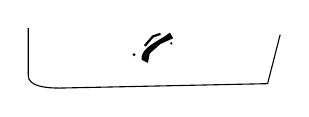
\begin{tikzpicture}[x=1cm,y=1cm,scale=.8]
\draw (0,.9)--(0,.15)..controls(0,-.03)and(.3,-.05)..(.5,-.05)--(3.8,.02)--(4,.8);
\fill (1.8,.4)..controls(1.78,.55)and(1.96,.65)..(2.15,.76)--(2.25,.83)--(2.3,.74)--(2.1,.65)--(1.93,.5)--(1.9,.35)--cycle;
\draw[line width=.8pt] (1.85,.62)--(1.98,.77)--(2.1,.81);
\fill(1.68,.48)circle(.025);\fill(2.27,.66)circle(.02);
\end{tikzpicture}}

\deleted{\uline{Proposition}}\inserted{Cor. 3} Soient $\deleted{F}G,F$ deux figures. Pour que $\deleted{F}G\subset F$\inserted{ (i.e. $G$ sous figure de $F$)}, il f et s. que $\deleted{F}G$ \uline{compatible} à $F$ (i.e. $\deleted{\unsure{G|F}}F\cup\deleted{F}G$ une figure, soit $\deleted{\unsure{F|G}}H$) et $\deleted{F}G\ll F$, i.e $G\subset\deleted{G'}F'$, $\deleted{\unsure{G|F}}F'$ sub. de $F$.

En effet, par \deleted{\unsure{Cont|Cond|C}} C 4, \deleted{comme}
\diagram{\begin{tikzcd}[ampersand replacement=\&,row sep=.15em,column sep=.25em]
F \& \subset \& H=F\cup G \\
F'\arrow[u,Rightarrow,"\text{subd.}"] \& {} \& {}\\
\tikz[baseline=-.5ex]\node[rotate=90,inner sep=0pt] {$\subset$}; \& {} \& {}\\
\deleted{\unsure{F|G}}G \& {} \& {}
\end{tikzcd}}
% The following calculation is written immediately to the right of the diagram.
\[
G\subset \underset{\deleted{\unsure{F'\cap H|G'\cap H}}}{\deleted{G'}F'\cap H}\ \deleted{\unsure{\subset G'\cap H|\subset F'\cap H}}\ \underset{\mathrm C\,4}{\mathrel{\tikz[baseline=-.35ex]\draw[line cap=round] (.35,.16) .. controls (.12,.18) and (.02,.08) .. (0,0) -- (1.18,0);}}\ F
\]
donc $G\subset F$.

En particulier, on trouve :
% slanted
\margin{C'est la partie sérieuse de C 4 \(\left(\vphantom{\dfrac{1}{1}}\right.\)}
\[
\text{Si } X\in M,\ F\in\mathcal F,\ \text{alors}\quad X\in F\ \Longleftrightarrow\
\left\{\begin{aligned}
&X\ \text{comp. à }F\\
&X\ \text{raffine }F
\end{aligned}\right.
\]
donc
\[
\text{Si } X,Y\in M,\ \text{alors}\quad X\leq Y\ \Longleftrightarrow\
\left\{\begin{aligned}
&X\ \text{comp. à }Y\\
&X\ \deleted{\text{raffine}}\ll Y
\end{aligned}\right.
\]

% slanted
\margin{\uline{NB} $F$ et $G$ disj. ssi $X\in F,\ Y\in G\Rightarrow X$ et $Y$ disj.$^{\mathrm{ts}}$ (i.e. ou non compatibles, \unsure{ou} $X$ et $Y$ \unsure{elt|et} \uuline{distincts})}

\deleted{\uline{\unsure{C 5|C 2}}} $F,G\in\mathcal F$ sont dites \uline{disjointes} si elles sont compatibles (i.e $F\cup G\in\mathcal F$) et $F\cap G=\varnothing$. On dit que $X,Y$ sont disjointes, ssi $F_X$ et $F_Y$ le sont i.e. $X$ et $Y$ compatibles, et $\nexists Z$ avec $Z\leq X,Y$.

Si $F$ et $G$ sont disjointes, alors pour $F'\subset F,G'\subset G$ sous-figures, elles sont disjointes. De plus ;

\cotefile{156-4}
\scanpage{50}
\mspage{49}

\deleted{\uline{Cont 5} Si $F$ et $G$ sont deux figures disjointes, et \unsure{si} $F'$, \deleted{$G'$\illegible{1} de} subdivision\unsure{s|{}}\unsure{,} \inserted{de $F$} alors $F'$ et $G$ sont disjointes.} \margin{\deleted{[\uline{NB} $F'\cap G$ est défini comme, c'est $F'$ et $G$ \uline{compatibles} qui est en cause.}}

\deleted{\uline{Cor} Si $F'$ raffine $F$, $G'$ raffine $G$, \deleted{alors} $F$ et $G$ disj. alors $F'$ et $G'$ disjointes.}

\margin{\begin{tikzpicture}[x=.5cm,y=.5cm]\draw(0,0)--(0,1.5);\draw(.13,0)--(.13,1.5);\end{tikzpicture}}\uline{C\deleted{\unsure{ont|ompt|onst}} 5} Soient $F$ une figure, $F'$ une subdivision de $F$. \deleted{\unsure{A}}Alors pour tt figure $G$, $G$ est disjointe ; $F$ ssi elle est disjoint\unsure{e} de $F'$

\uline{NB} Il suffit de le poser pour $G$ élémentaire.

Il résulte alors de \deleted{\uline{Cont 4}} C4 que $F'\cup G$ est une subdivision de $F\cup G$.

\uline{Cor} Soient $F$ et $G$ figures disjointes, alors pour $F'\ll F$, $G'\ll F$, $F'$ et $G'$ sont disjointes, et $F'\cup G'\ll F\cup G$. Si $F'$ et $G'$ sont des subd de $F,G$, alors $F'\cup G'$ en est une de $F\cup G$.

\margin{\begin{tikzpicture}[x=.5cm,y=.5cm]\draw(0,0)--(0,1.5);\draw(.13,0)--(.13,1.5);\end{tikzpicture}}\uline{C 6} (Subdivisions induites) Soient $F$ une figure, $F'$ une subdivision de $F$, $G$ une sous-figure de $F$. Alors il existe une unique subdivision $G'$ de $G$, telle que
\[G'\subset F'\]
(subdivision induite) \inserted{et $G'$ est formée des $X\in F'$ telles que $X\ll G$}
\figure{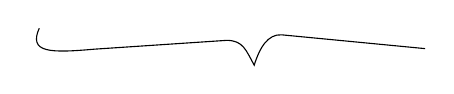
\begin{tikzpicture}[x=1cm,y=1cm,scale=.7]
\draw (0,.25)..controls(-.2,-.2)and(.2,-.2)..(1,-.13)--(3.4,.03)..controls(3.7,.03)and(3.75,-.15)..(3.9,-.42)..controls(4,-.1)and(4.15,.15)..(4.4,.13)--(7,-.12);
\end{tikzpicture}}

\margin{NB \inserted{Double} Transitivité de l'induction. \uline{Notation} $F'|G$}

\margin{\begin{tikzpicture}[x=.5cm,y=.5cm]\draw(0,0)--(0,1.5);\draw(.13,0)--(.13,1.5);\end{tikzpicture}}\uline{C 7} (\deleted{\unsure{D|R}}Recollement des subdivisions) Soit $F$ une figure, \deleted{\unsure{chaque} \illegible{3} tt} \inserted{$F_i$ des sous-figures} \deleted{$X\in$} telles que $F=\bigcup F_i$. Soit, pour tt $i$, $F'_i$ une subdivision de $F_i$, et supposons

\scanpage{51}
\mspage{50}

que \unsure{pour|\deleted{pour}} $i,j\in I$, $\unsure{i\Rightarrow j|i\ne j}$, $F'_i|F_i\cap\deleted{G}F_j=\deleted{G}F'_j|F_i\cap F_j$

Alors il existe une unique subdivision $F'$ de $F$ telle que $F'|F_i=F'_i\quad\forall i\in I$

\uline{Cor} Pour que deux subdivisions \inserted{$F',F''$ de $F$} soient égales, il f et s qu'elles induisent la $=$ subdivision sur chaque sous-figure élémentaire $F_X$ .ie sur chaque multistrat.

\deleted{\uline{Cor}} \uline{Proposition} \deleted{\unsure{1|a}}) Soient $F$ une figure, $G$ une sous-figure, $\deleted{G}F'$ un raffinement de $F$, et $G'=\{X\in F'\mid X\ll G\}$ c'est donc une sous figure de $F'$, \deleted{et} \inserted{Je dis qu'}elle raffine $G$ et c'est \inserted{\unsure{disons|\deleted{d'ailleurs}|\deleted{même}}} la plus grande sous-figure de $F'$ qui raffine $G'$.

% slanted
\margin{\uline{raffinement} \uline{induit}. \uline{NB} Si $\deleted{G}F'\subset\deleted{G}F$, alors $G'$ n'est autre que l'intersection $F'\cap G'$.}

\diagram{\begin{tikzcd}[ampersand replacement=\&,column sep=small,row sep=small] \deleted{G}F' \arrow[r,phantom,"\ll" description] \arrow[d,phantom,"\cup" description] \& F \arrow[d,phantom,"\cup" description] \\ G' \arrow[r,phantom,"\ll" description] \& G \end{tikzcd}}

\deleted{Ceci dit,} Il y a qque chose à prouver, car le seul fait que les $X\in G'$ raffinent $G$ n'implique \unsure{ps|pas} que $G'$ raffine $G$. Mais on a une \deleted{raffinement} \inserted{subdiv.} $\overline{F''}$ de $F$ tel que \diagram{\begin{tikzcd}[ampersand replacement=\&,column sep=small,row sep=small] F' \arrow[r,phantom,"\subset" description] \& \overline{F''}\arrow[r,"\sim","s."' ]\arrow[d,phantom,"\cup" description] \& F\arrow[d,phantom,"\cup" description] \\ \& \overline{G''}\arrow[r,"\sim","s"' ] \& G \end{tikzcd}} considérons la subd. induit \deleted{sur} $G$\inserted{(C,6)}, $\overline{G''}$, formée des $X\in\overline{F}$ telles que $X\deleted{\unsure{\in|\subset}}\ll \deleted{F}G$. \deleted{Ceci} Par définition, on a donc $G'=F'\cap G'$, qui est \deleted{bien} une sous-figure de $\overline{\deleted{\unsure{C}}G''}$ donc raffine $G$.

\scanpage{52}
\mspage{51}

\uline{Corollaire} Sous les conditions précédentes, $G'$ est le $\mathrm{Inf}$ de $F'$ et $G$, dans l'ens des figures pour la \deleted{notion} \inserted{relation} de raffinement. En d'autres termes, \deleted{\unsure{tout|toute|tt}} figure \inserted{$\Phi$} qui raffine à la fois $F'$ et $\deleted{\unsure{F}}G$, raffine $G'$\figure{\begin{tikzpicture}\draw (0,0)--(0,1.8);\end{tikzpicture}}

\diagram{\begin{tikzcd}[ampersand replacement=\&,column sep=small,row sep=small,execute at end picture={\draw (\tikzcdmatrixname-1-1.west) -- (\tikzcdmatrixname-1-2.north east); \draw (\tikzcdmatrixname-2-3.south west) -- (\tikzcdmatrixname-1-4.north east); \draw (\tikzcdmatrixname-2-4.south west) -- (\tikzcdmatrixname-1-5.north east); \draw (\tikzcdmatrixname-2-5.south west) -- (\tikzcdmatrixname-1-6.west);}] \deleted{\Phi} \& \deleted{\unsure{\Phi\subset\Phi|G\subset\Phi}} \& \deleted{\unsure{\overline{F}'}} \arrow[r,"\deleted{\sim}"] \arrow[d,phantom,"\deleted{\cup}" description] \& \deleted{F'} \arrow[r,phantom,"\deleted{\subset}" description] \arrow[d,phantom,"\deleted{\cup}" description] \& \deleted{\overline{F''}} \arrow[r,"\deleted{\sim}"] \arrow[d,phantom,"\deleted{\cup}" description] \& \deleted{F} \arrow[d,phantom,"\deleted{\cup}" description] \\ \& \& \deleted{\overline G'} \arrow[r,"\deleted{\sim}"] \& \deleted{\deleted{F}G'} \arrow[r,phantom,"\deleted{\subset}" description] \& \deleted{\overline{G''}} \arrow[r,"\deleted{\sim}"] \& \deleted{G} \end{tikzcd}}

On utilise que $F\subset\overline{F'}$, où $F''$ subd. de $F$, et que $\Phi\subset\overline{F} '$, où $\overline F'$ subd. de $F'$, \deleted{et que}

\diagram{\begin{tikzcd}[ampersand replacement=\&,column sep=small,row sep=small] \& \& \deleted{\widetilde F}\arrow[d,"\deleted{\unsure{\subset|\swarrow}}" description,phantom]\arrow[dr,"\sim"] \& \& \\ \Phi\arrow[r,phantom,"\subset" description] \& \overline F'\arrow[r,dash,"\sim"]\arrow[d,phantom,"\cup" description] \& F'\arrow[r,phantom,"\subset" description]\arrow[d,phantom,"\cup" description] \& \overrightarrow F\arrow[r,"\sim"]\arrow[d,phantom,"\cup" description] \& F\arrow[d,phantom,"\cup" description] \\ \& \overline G'\arrow[r,"\sim"] \& G'\arrow[r,phantom,"\subset" description] \& \overline G\arrow[r,"\sim"] \& G \end{tikzcd}}

On va prouver que $\Phi\subset\overline G'$\inserted{(\deleted{\unsure{dont|donc}} $\Phi\ll G'$)}. Soit $X\in\Phi$, on a $X\in\overline F'$, \deleted{et $X$} il faut prouver $X\in\overline{G'}$, i.e. \deleted{$\unsure{\overline{F}'|G'}$} que tt élément de $\overline{F'}$ \uline{qui raffine} $G$, est dans $\overline G'$. Mais $\overline F'$ \uline{est \unsure{induite|induit} par une} subd. $\widetilde F$ de $F$ (C 4 revu et corrigé -- cf son cor.) donc $\overline F'\subset\widetilde F\xrightarrow{\sim}\overrightarrow F$, donc $X\in\widetilde F$ et $X$ raffine $G$, donc \deleted{$X\in\widetilde F'$} $X\in\widetilde G$, subd. de $G$ induite par la \unsure{subd.} $\widetilde F$ de $F$, donc

\diagram{\begin{tikzcd}[ampersand replacement=\&,column sep=small,row sep=small] \overline F'\arrow[r,phantom,"\subset" description] \& \widetilde F\arrow[r,"\sim"]\arrow[d,phantom,"\cup" description] \& \overrightarrow F\arrow[r,"\sim"]\arrow[d,phantom,"\cup" description] \& F\arrow[d,phantom,"\cup" description] \\ \& \widetilde G\arrow[r,"\sim"] \& \overline G\arrow[r,"\sim"] \& G \end{tikzcd}}

\deleted{$\Phi$} $X\in\overline F'\cap\widetilde G=\overline G'$, qed, ouf ! (C'était l'ancien Cont 8)

\diagram{\begin{tikzcd}[ampersand replacement=\&,column sep=small,row sep=small,execute at end picture={\draw (\tikzcdmatrixname-2-2.south) -- ([xshift=-3pt,yshift=8pt]\tikzcdmatrixname-4-2.north) .. controls ([xshift=-3pt,yshift=2pt]\tikzcdmatrixname-4-2.north) and ([xshift=2pt,yshift=2pt]\tikzcdmatrixname-4-2.north) .. ([xshift=5pt,yshift=9pt]\tikzcdmatrixname-4-2.north);
\draw (\tikzcdmatrixname-2-4.south) -- ([xshift=-3pt,yshift=8pt]\tikzcdmatrixname-4-4.north) .. controls ([xshift=-3pt,yshift=2pt]\tikzcdmatrixname-4-4.north) and ([xshift=2pt,yshift=2pt]\tikzcdmatrixname-4-4.north) .. ([xshift=5pt,yshift=9pt]\tikzcdmatrixname-4-4.north);
\draw (\tikzcdmatrixname-3-3.south) -- ([xshift=-3pt,yshift=8pt]\tikzcdmatrixname-4-3.north) .. controls ([xshift=-3pt,yshift=2pt]\tikzcdmatrixname-4-3.north) and ([xshift=2pt,yshift=2pt]\tikzcdmatrixname-4-3.north) .. ([xshift=5pt,yshift=9pt]\tikzcdmatrixname-4-3.north);
\draw (\tikzcdmatrixname-3-5.south) -- ([xshift=-3pt,yshift=8pt]\tikzcdmatrixname-4-5.north) .. controls ([xshift=-3pt,yshift=2pt]\tikzcdmatrixname-4-5.north) and ([xshift=2pt,yshift=2pt]\tikzcdmatrixname-4-5.north) .. ([xshift=5pt,yshift=9pt]\tikzcdmatrixname-4-5.north);
\draw ([yshift=-5pt]\tikzcdmatrixname-3-5.south) .. controls ([xshift=0pt,yshift=-12pt]\tikzcdmatrixname-3-5.south) and ([xshift=2pt,yshift=-12pt]\tikzcdmatrixname-3-5.south) .. ([xshift=5pt,yshift=-7pt]\tikzcdmatrixname-3-5.south);
\draw (\tikzcdmatrixname-1-1.south west)--(\tikzcdmatrixname-1-2.north east);
\draw ([xshift=-3pt]\tikzcdmatrixname-4-1.west) .. controls ([xshift=-16pt,yshift=43pt]\tikzcdmatrixname-2-1.west) and ([yshift=14pt]\tikzcdmatrixname-1-2.north) .. ([yshift=10pt]\tikzcdmatrixname-1-3.north) .. controls ([xshift=38pt,yshift=10pt]\tikzcdmatrixname-1-5.north) and ([xshift=15pt]\tikzcdmatrixname-4-5.east) .. ([xshift=4pt]\tikzcdmatrixname-5-5.south east);}] \deleted{F'}\arrow[r,dash] \& \deleted{F'} \& \widetilde F\arrow[dr,"\sim"]\arrow[d,dash] \& \& \vphantom{F} \\ \Phi\arrow[r,hook] \& \overline F'\arrow[ur,hook]\arrow[dr,"\sim"] \& {} \& \overrightarrow F\arrow[dr,"\sim"] \& \\ \& \& F'\arrow[ur,hook]\arrow[dd,dash,bend right=13] \& \& F \\ \vphantom{G} \& \overline G'\arrow[dr,"\sim"]\arrow[r,phantom,"\rotatebox{35}{$\subset$}" description] \& \widetilde G\arrow[r,"\sim"] \& \overline G\arrow[r,"\sim"] \& \substack{\unsure{\deleted{G}|G}\\G} \\ \& \& G'\arrow[ur,phantom,"\rotatebox{40}{$\subset$}" description] \& \& \vphantom{G} \end{tikzcd}}

\scanpage{53}
\mspage{52}

\uline{13 juin} On n'a pas encore exprimé tous les Axiomes \uline{Cont}. 1, ...., il reste pour compte

\uline{Cont} 3 dim finie

\uline{Cont} 4 ``admissibilité'' -- mais résulte déjà je crois des axiomes C.

\uline{Cont} 6 \inserted{Critère de} disjonction via les lieux -- on y reviendra.

\uline{Cont} 7 Deux lieux de str. dominantes différentes sont disjoints.

Mais avant de continuer, je voudrais encore une fois changer d'optique !

Prendre comme ens de base $\mathcal F$, l'ens des figures, avec les deux relations d'ordre \[ \leq\ \text{(ou l'inclusion)} \qquad \text{et}\qquad \preccurlyeq\ \text{(la subdivision)} \]

\uline{Contrée} (quatrième mouture !)

\unsure{$U$ est|C'est} un ens. $\mathcal F$ d'objets, appelés \uline{figures}, et deux relations d'ordre $\leq$ et $\preccurlyeq$ sur $\mathcal F$ : \[ \mathcal C=(\underline{\mathcal F},\leq,\preccurlyeq) \] satisfaisant à des axiomes\unsure{,|{}} qu'on va énumérer. Si $F$ et $G$ sont deux figures et $F\leq G$, on dit que $F$ est une \uuline{sous}-\uline{figure}, et on écrira aussi souvent $F\subset G$. Si $F\preccurlyeq G$, on dit que $F$ est une \uline{subdivision} de $G$, ou que $F$ subdivise $G$.

\scanpage{54}
\mspage{53}

D'abord, on va dégager les axiomes pour $\leq$

\uline{$\mathcal C$ 1} a) $\mathcal F\ne\varnothing$

\deleted{\uline{\unsure{C 2}}} b) Si $F\in\mathcal F_{\leq}$, et $(F_i)_{i\in I}$ est une famille d'objets de $\mathcal F$ avec $F_i\leq F$, alors $\underset{i}{\mathrm{Sup}}\,F_j$ existe. (Toute famille majorée de figures a une borne sup.)\figure{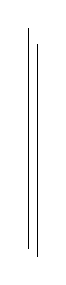
\begin{tikzpicture}\draw (0,0)--(0,2.8);\draw (.12,-.1)--(.12,2.6);\end{tikzpicture}}

\uline{Corollaire} $\mathcal F$ a un plus petit élé\deleted{\unsure{ment|mt}} (savoir, le $\mathrm{Sup}$ de la famille vide d'objets)

\uline{NB} En présence de \deleted{\unsure{C2}} \uline{C 1 b)}, la validité de a) \uline{équivaut} à celle du corollaire.

Le plus petit \unsure{élémt|élément} est appelé \uline{figure vide}, notée $\varnothing_{\mathcal F}$ ou simplement $\varnothing$, par abus de langage, et si confusion n'est à craindre

\figure{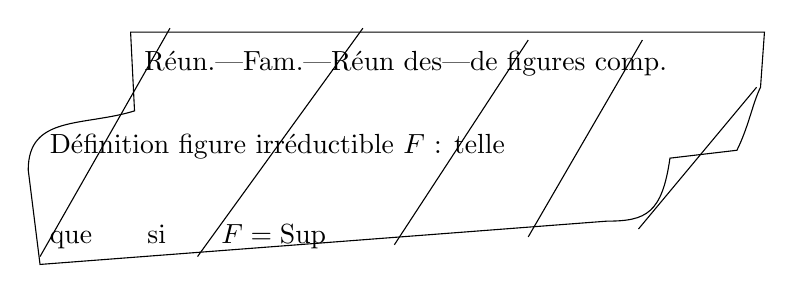
\begin{tikzpicture}[x=1cm,y=1cm]
\node[anchor=west] at (1.2,2.2) {\deleted{\unsure{Réun.|Fam.|Réun} \unsure{des|de} figures comp.}};
\node[anchor=west] at (0,1.15) {\deleted{\uline{Définition} \uline{figure} \uline{irréductible $F$ : telle}}};
\node[anchor=west] at (0,0) {\deleted{que\qquad si\qquad $F=\mathrm{Sup}$}};
\draw (1.15,2.6)--(9.2,2.6)--(9.15,1.9) .. controls (9.05,1.7) and (9.0,1.4) .. (8.85,1.1) -- (8.0,1.0) .. controls (7.9,.3) and (7.7,.2) .. (7.2,.2) -- (0,-.35)--(-.15,.85) .. controls (-.15,1.55) and (.55,1.4) .. (1.2,1.6)--cycle;
\draw (0,-.25)--(1.65,2.65) (2.0,-.25)--(4.1,2.65) (4.5,-.1)--(6.2,2.5) (6.2,0)--(7.65,2.5) (7.6,.1)--(9.1,1.9);
\end{tikzpicture}}

Figures \uline{compatibles}, ens de figures \deleted{\unsure{compatibles}} compatibles : \deleted{\unsure{un qui|qui}} \inserted{dans leur ens.} (ou \uline{configuration}) : qui est majoré pour $\leq$. \margin{P} Figure engendrée, ou \uline{réunion} ($F\vee G$, $\bigvee_i f_i$, $\mathrm{Sup}\,F_i$, parfois noté $F\cup G$ \unsure{ou|--} $\deleted{F}\bigcup_iF_i$ cf plus bas).

\uline{Déf} \uline{Figure irréductible} $F$ : telle que $\displaystyle F=\underset{i\in I}{\mathrm{Sup}}\,F_i\ \overset{-}{\Longrightarrow}\ \exists i\in I,\ F_i=F$.

\deleted{\uline{C 2}} Les figures irréductibles sont appelées des \uline{multistrates}. \inserted{L'ens des multistrates noté $ M$} Les figures irréductibles

\scanpage{55}
\mspage{54}

majorées par $F$ s'appellent les \uline{strates} de $\deleted{E}F$. (Donc, \deleted{des} strate de $F$ est une multistrate)

L'ens des strates de $F$ \deleted{s'appelle} sera noté $\overline F$ : \[ \begin{aligned} \deleted{\overline F\subset M} &\qquad  M\subset\mathcal F\\ F\longrightarrow\overline F &\qquad \mathcal F\longrightarrow\mathcal P( M). \end{aligned} \]

\uline{$\mathcal C$ 2} Toute figure est la borne supérieure de ses strates : \[ F=\underset{\deleted{A}X\in\overline F}{\mathrm{Sup}}\ X \]
\figure{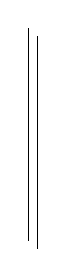
\begin{tikzpicture}\draw (0,0)--(0,2.7);\draw (.12,-.1)--(.12,2.6);\end{tikzpicture}}
\uline{Corollaire} 1 L'application $\deleted{X}F\longrightarrow\overline{\deleted{C}F}$ \[ \mathcal F\longrightarrow\mathcal P( M) \] est injection, et induit un iso d'ens ordonnés de $\mathcal F$ avec l'ens $\Phi\subset\mathcal P( M)$ formé des $\overline F$.

Cet iso. transforme $\underset{i}{\mathrm{Sup}}$ en $\bigcup_i$
\figure{\begin{tikzpicture}\draw (0,1.5)--(0,2.8);\draw (.1,-2)--(.1,.5);\end{tikzpicture}}
\uline{Corollaire 2} L'ens $\Phi$ des parties de $ M$ satisfont les deux conditions,

\deleted{a) $\Phi\ne\varnothing$}

% slanted
\margin{\deleted{Ceci}} \deleted{b)}a) Si $A\in\Phi$, et $(A_i)_{i\in\unsure{I|\Phi}}$ est une famille d'éléments de $\Phi$, avec $A_i\subset A$, alors $\bigcup_iA_i\in\Phi$.

b) $\forall X\in M$, il existe un plus petit $A=A_X$ tel que $X\in\unsure{A|A_x|A_X}$ (a fortiori, $\Phi$ recouvre $ M$).

\scanpage{56}
\mspage{55}

c) $\varnothing\in\Phi$ \deleted{$\ne\varnothing$ [en vertu de b), c'est tjrs vrai si $ M\ne\varnothing$], et si $ M=\varnothing$, cela signifie que $\varnothing$}

\deleted{\uline{\unsure{Rép.|Rq.}} (équivaut : $\varnothing\in\Phi$)}

\uline{Remarque} Inversement, soient $ M$ un ens, $\deleted{\Phi}\mathcal F\subset\mathcal P( M)$ satisfaisant les conditions a) b) c). NB La condition c résulte de \inserted{a),} b si $ M\ne\varnothing$. Dans tous les cas, elle équivaut à : \deleted{\unsure{$\in$|à}} c') $\deleted{\Phi}\mathcal F\ne\varnothing$ i.e existe $\deleted{X}A\subset M$ telle que $A\in\deleted{\Phi}\mathcal F$

% slanted
\margin{\unsure{Ces|Les} conditions impliquent que $\mathcal F$ est stable par $A\cap B$ (mais en général \unsure{on n'a|\ldots} $\not\Rightarrow$ $ M\in\mathcal F$ !)}

Alors

1°) $\Phi$ ordonné par inclusion \deleted{\unsure{ad|sa}}satisfait les conditions C1, C2. \deleted{Les objets irréductibles} \deleted{\unsure{sont}}

2°) Les objets irréductibles sont les $A_X$, et $X\mapsto\deleted{X}A_X$ est une bijection de $ M$ \deleted{avec} l'ens des objets irred. de $\deleted{\Phi}\mathcal F$.

3°) Si $X\in M$, $A\in\deleted{\Phi}\mathcal F$, alors $X\in A\Longleftrightarrow A_X\subset A$ \deleted{, donc} (tautologique) donc \deleted{$A\in\mathcal F$} si on identifie $ M$ \inserted{(par $X\unsure{\vdash|\mapsto} A_X$)} à l'ens des objets irréductibles de $\deleted{\Phi}\mathcal F$, alors pour $A\in\mathcal F$, $\overline A=\{A_X\mid A_X\subset A\inserted{\text{ie.}\,X\in A}\}$ s'identifie à $A$ lui-$=$.

\centerline{\rule{1.8cm}{0.35pt}}

On considérera $ M$ comme ordonné par $\leq$ (jamais par $\prec$ !) : multistrates et \uline{sous-multistrates}. Les figures \inserted{$F$} peuvent s'identifier aux \deleted{des parties} ens. de multistrates $\overline F$ correspondants (\unsure{ch. que|cl. par|chaque} figure à l'ens de ses strates).

\scanpage{57}
\mspage{56}

\uline{Proposition} a) Si $F$ \deleted{\unsure{est|était}} est une figure, alors les figures $F'$ telles que $F'\leq F$ s'identifient, par l'application $F'\mapsto\overline F'$, aux parties de $\overline F$ qui sont \uline{fermées} pour la relation d'ordre \inserted{$\leq$} de $M$.

b) Si $F$ et $G$ sont deux figures, $F\wedge G$ existe (inf pour $\leq$) \inserted{\uuline{figure intersection}} et \deleted{\unsure{on|en}} $\overline{F\cap G}=\overline F\cap\overline G$. Même pour une famille $(F_i)_{i\in I}$ quelc. \inserted{avec 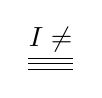
\begin{tikzpicture}[baseline=(f.base)]\node[inner sep=0] (f) {$I\neq\varnothing$};\draw ([yshift=-2pt]f.south west)--([yshift=-2pt]f.south east);\draw ([yshift=-4pt]f.south west)--([yshift=-4pt]f.south east);\draw ([yshift=-6pt]f.south west)--([yshift=-6pt]f.south east);\end{tikzpicture}}.

% Two marginal callout strokes, reproduced beside the associated additions.
\figure{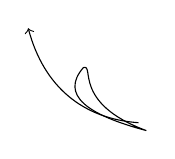
\begin{tikzpicture}[x=1cm,y=1cm]
\draw[->] (1.4,0) .. controls (.7,.05) and (.2,.45) .. (0,1.2);
\draw (1.5,-.1) .. controls (.55,.25) and (.85,.75) .. (.7,.7) .. controls (.4,.35) and (.75,.1) .. (1.5,-.1);
\end{tikzpicture}}
% margin note written sideways
\margin{\uline{Mais attention} il vaut mieux ne pas les noter $F\cap G$, car quand il y a une notion de support, ça ne correspond pas à l'intersection des supports, sauf si $F,G$ compatibles.}

[ \uline{Lieux} de $\mathcal F$ : ce sont les \deleted{\unsure{pas|pet}} figures qui sont \uline{minimales} dans $\mathcal F\setminus\{\varnothing_{\mathcal F}\}$. \deleted{Un,} \deleted{Un lieux est de \unsure{ce nom|nom}}  Tout lieu est irréductible. Donc les lieux sont aussi les éléments minimaux de $ M$ : ce sont les multistrates qui n'ont d'autres strates qu'elles-même. ] \deleted{Si $F$ est une figure, les}

% slanted
\margin{Définition courante n'est raisonnable que dans certains cas \deleted{(quand les} (p. ex. les contrées en boules'', ou contrées par morceaux $\ldots$) Car dans les cas types d'ordre quelconq., un \unsure{modèle|modélé} $\overline E$ \unsure{de str.|de structure} \unsure{semi-}\illegible{1} \inserted{\unsure{univers vides|univers vide},} forme \deleted{\unsure{peut être une|peut être un}} \inserted{une} multistrate \unsure{minimale|minime}, mais on ne \unsure{l'appelle|appelle} un ``lieu'' que si elle est \unsure{vide réel|vide réelle} !}

\uline{Figures} \uline{disjointes} \unsure{,,|''} \uline{$F$} et \uline{$G$} : telles que a) $F$ et $G$ compatibles, i.e $F\cup G$ existe \deleted{et b)} ou encore $\{F,G\}$ majoré pour $\leq$ et b) $F\cap G=\varnothing_{\mathcal F}$ \deleted{\unsure{ou|et} Cela signifie \unsure{donc|que}} \inserted{(i.e. $\overline F\cap\overline G=\varnothing$)}.

% Long curved separator beside the lower margin and proposition.
\figure{\begin{tikzpicture}[x=1cm,y=1cm]\draw (.6,3) .. controls (.2,2.3) and (.05,1.3) .. (.15,.9) .. controls (.2,.3) and (.4,.05) .. (.65,0);\end{tikzpicture}}
% slanted
\margin{bloque mes ``\unsure{coproduits|composantes}''}

\deleted{Si $F$ et $G$ sont} \uline{Prop} Si $F$ et $G$ sont disjointes, alors pour $F'\leq F$, $G'\leq G$, $F'_{a}$ et $G'$ sont disjointes, et $F'\cup G'$ est une sous figure de $F\cup G$, l'application $(F';G')\mapsto F'\cup G'$ est une bijection \deleted{de l'ens de $\unsure{\mathcal F|F}$}

\cotefile{156-4}
\scanpage{58}\mspage{57}
\diagram{\begin{tikzcd}[ampersand replacement=\&,column sep=large]
\underset{\substack{\text{ss-fig de}\\ F}}{\mathcal F_{\leq F}}
 \times
\underset{\substack{\text{ss fig}\\ \text{de }G}}{\mathcal F_{\leq G}}
 \arrow[r,"\sim"] \&
\underset{\substack{\text{ss. fig}\\ \text{de }F\cup G=H}}{\mathcal F_{\leq F\cup G}}
\end{tikzcd}}

(On récupère $F',G'$ : partir de $H'=F'\cup G'$ comme $H\cap F$ et $H\cap G$.) Item pour une \deleted{\unsure{familles|famille} mutuellement disjointes d'une} \inserted{des figures deux à deux disjointes \unsure{fais.t une|ds une}} configuration (famille pas \unsure{néc.t|néct} finie). \deleted{figure (\unsure{y}}

\uuline{Démonstration} \unsure{Particulièrt|Particulièrmt} claire, quand on interprète $\mathcal F$ en termes de l'ens $\Phi\subseteq\mathcal P(M)$ satisfaisant à a) b) c). L'ens ordonné $M_{\leq F\vee G}$ s'identifie à la réunion disjointe dans l'ens ordonné somme de $M_{\leq F}$ et $M_{\leq G}$, donc ses parties fermées \deleted{sont} s'en définies par les couples de parties fermées de $M_{\leq F}$ et $M_{\leq G}$ \ldots

\uline{Remarque}
% slanted
\margin{à joindre à la remarque de la page 55}
En termes de l'ens \uline{ordonné} $M$, la donnée de $\Phi$ équivaut : un ens de parties \uline{fermées} de $M$, satisfaisant
\[
\begin{aligned}
\text{a) }&\deleted{\Phi}\forall\,\deleted{\unsure{=}}A\in\Phi,\quad
 \deleted{\text{toute}}\inserted{\text{et}}\ \text{partie fermée }A'\text{ de }A,\ \text{on a }A'\in\Phi\\
&\deleted{\text{b) }\varnothing\in\Phi\quad
 (\Longleftrightarrow\Phi\ne\varnothing,\ \text{compte tenu de a), et}}\\
\text{b) }&\bigcup_{A\in\Phi} A=M\quad\deleted{\unsure{\forall x}}\quad
 \left[\,\underset{\substack{\text{à cause}\\\text{de a)}}}{\Longleftrightarrow}\
 \forall x\in M,\ M_{\leq x}\in\Phi\,\right]\\
\text{c) }&\varnothing\in\Phi\quad
 \bigl(\underset{\deleted{\unsure{\text{a)}|\text{a) b)}}}}{\Longleftrightarrow}
 \Phi\ne\varnothing,\ \text{et \unsure{automatiqt} satisfaite}\ \deleted{\unsure{\Phi}}\\
 &\hspace{7em}\text{(à cause de b)) si }M\ne\varnothing\bigr)
\end{aligned}
\]

\uuline{NB} Soit $\mathcal P_f(M)$ l'ens des parties \uline{fermées} de $M$, $\mathcal P_{f'}(\mathcal F)$ de $\mathcal F$ qui sont stables par Sup. Si $\mathcal F'$ et $M'$ se correspondent \margin{TSVP}, 
\diagram{\fbox{\begin{tikzcd}[ampersand replacement=\&,column sep=large]
\mathcal P_f(\unsure{\mathcal F|M\mathcal F}) \arrow[r,shift left=.6ex,"\varphi"] \& \mathcal P_f(M) \arrow[l,shift left=.6ex,"\psi"]
\end{tikzcd}}}
$\varphi(\mathcal F')=\mathcal F'\cap M$, $\psi(M')=\{F\in\mathcal F\mid\overline F\subset \unsure{M'|M}\}$ alors $\varphi,\psi$ bij. inverses l'une de l'autre

\scanpage{59}\mspage{58}
% slanted
\margin{alors $\mathcal F'$ satisfait aussi $C1$, $C2$, et $M'$ \deleted{\unsure{s'identifie}} \inserted{\unsure{désignant|désigne|désignant par}} ses objets irréductibles, la relation d'ordre (de $M'\unsure{)|{}}$ induite par $\mathcal F'$ étant celle \deleted{\unsure{d'}}induit par $M$. Si $\mathcal F$ satisfait $C3$, alors $\mathcal F'$ aussi.}\margin{\begin{tikzpicture}[x=1cm,y=1cm]\draw[<->] (.1,.55) .. controls (.7,.5) and (.1,.1) .. (.8,0);\draw (-.1,-.18)--(1.45,-.18);\end{tikzpicture}}

\deleted{\mbox{\uline{C 3}} Soient $F,G,H$} \deleted{trois} \deleted{figures entre elles compatibles.} \deleted{\mbox{\inserted{i.e. deux à deux \unsure{majorés.|majorées.}}}} \deleted{Alors $\{F,G,H\}$ est une configuration i.e.} \deleted{$F,G,H$} \deleted{$\exists$ figure $K$ telle que $F,G,H$ sont des sous figures de $K$ (donc existe borne supérieure de}

\uline{C 3} Soient $F,G\in\mathcal F$, telles que
\[
\forall\,x\in\overline F,\ \overleftarrow{y}\in\overline G,\quad x\text{ et }y\text{ compatibles}
\]
\margin{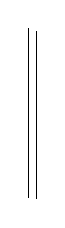
\begin{tikzpicture}[x=1cm,y=1cm]\draw (0,0)--(0,2.15);\draw (.1,-.02)--(.1,2.12);\end{tikzpicture}}Alors $F$ et $G$ sont compatibles

% slanted
\margin{\uline{Cor} Pour que $F,G$ disjointes, il f et s. que $\forall x\in\overline F,y\in\overline G$, $x$ et $y$ le soient}

\uline{NB} L'inverse évident : Si $F$ et $G$ sont compatibles, alors pour toutes sous figures $F'$ de $F$ (p. ex. une ss-fig. él.) et $G'$ de $G$ (idem) $F'$ et $G'$ le sont

\uline{Cor} Soient $F$ et $G,H$ \deleted{deux} figures, \deleted{Si} avec $F,G$ compatibles. Pour que $H$ soit compatible : $F\cup G$, il f et s qu'il le soit : $F$ et : $G$. \deleted{Deux}

Plus gén, soit $(F_i)_{i\in I}$ une configuration, $F$ la \deleted{\unsure{leur|borne}} \inserted{figure} réunion. Pour que $H$ soit compatible : $F$, il f et s que $H$ soit compatible avec $F_i$.

\scanpage{60}\mspage{59}
Donc, en \deleted{\unsure{de|te}}termes d'une structure portée par un ens ordonné $M$ (cf remarque page 58, on trouve ceci. On a sur \deleted{\uline{Définition}} $M$ une relation $R$ (``compatibilité) qui est réflexive symétrique (donc équivaut à la donnée de $\mathcal S\subset\mathcal P_2(M)$), \deleted{\uline{impliquant}}\inserted{et telle que} $R(x,y)$ implique $R(x',y')$ pour $x'\leq x$, $y'\leq y$. \deleted{\unsure{comp stable} par $\leq$.} Cela permet, à peu de choses près, de reconstituer $(\mathcal F,\leq)$, en \unsure{tant qu'}ens de parties de $M$. Pour l'expliciter,

Quelques terminologies

``\uline{Composante}'' \uline{irréductible} \inserted{(ou strate maximale)} d'une figure $F$ : \deleted{\unsure{o|a}}strate maximale de $F$ ($\exists$ tjrs si l'ens $\overline F$ des strates de $F$ est fini \inserted{(on dit alors que $F$ est une \uline{figure finie})} et $F\ne\varnothing_{\mathcal F}$).

Figure \deleted{de type}\inserted{de type fini} fini : qui est borne sup. de \unsure{l'ens|la réu} de ses ``composantes'' irréductibles (\unsure{exemple|exemples} : toute figure finie est de t.f.), ou encore, toute figure \inserted{$F$} qui est \deleted{de la forme $\operatorname{Sup}X$}\inserted{borne supr. d'un \unsure{nb} \uline{fini} de} figures irréductibles. \deleted{Ceci} (NB Dans les cas les plus importants, toute figure est finie, et a fortiori de type fini.)

Ceci dit, si $\mathcal F_{\mathrm{t.f.}}$ désigne l'ens figures de type fini, on récupère $\overline{\mathcal F_{\mathrm{t.f}}}$, l'ens des parties \unsure{correspondantes|correspondants} de $M$, par la seule connaissance de $(M,\leq,R)$,

\scanpage{61}\mspage{60}
de la façon suivante : ce sont les $A\in M$ tels que $A=\bigcup_i A_{x_i}$, où \deleted{les} $\{x_i\}$ \deleted{sont}\inserted{est} un ens fini d'éléments de $M$, mutuellement compatibles (\deleted{\unsure{pour}}\inserted{au sens de} $R$.).

Donc une structure $(\mathcal F,\leq)$ satisfaisant $\deleted{\unsure{C_1}}C1,\deleted{\unsure{C_2}}C2,\deleted{\unsure{C_3}}C3$ + figures \deleted{toutes} de type fini, équivaut à $(M,\leq,R)$, où \inserted{$R$ \uline{rel. sym. refl.}} \deleted{$(M,\leq)$}\inserted{où $\leq$ et $R$} satisfont \deleted{deux} conditions.

a) \inserted{(concernant $\leq$)} Pour tte partie fermée \uline{majorée} $A$\deleted{\unsure{,}} de $M$, $A$ est de type fini i.e de la forme $\bigcup_{\deleted{x_i}i}\deleted{A_{x_i}}M_{\leq\unsure{x_i|x}}$, où les $x_i\in A$ \deleted{\unsure{fo}} sont un ens fini [ pour ceci, il suffit que les $M_{\leq x}$ soient finis ]

% slanted
\margin{donc \unsure{toute|tte} partie fermée d'une partie fermée de type fini est de type fini}

b) (concernant $\leq$ \uline{et} $R$) Si $(x,y)\in R$, et $x'\leq x$, $y'\leq y$, alors $\deleted{R}(x',y')\in R$.

% slanted
\margin{C'est la propriété Cont 2 de \unsure{page|pg} 33}

(Les ``figures'' de $M$ sont alors les parties \deleted{fermées}\inserted{$A$} de $M$ qui ont les propriétés suivantes :
\[
\begin{aligned}
\text{a) } & A\text{ est fermé}\\
\text{b) } & A\text{ est de type fini}\\
\text{c) } & \deleted{\unsure{A}}\forall\,x,y\in A,\ \text{on a}\quad (x,y)\in R.
\end{aligned}
\]

\scanpage{62}\mspage{61}
\deleted{Soit} Ainsi, les \unsure{systèmes|système} $(\mathcal F,\leq)$ satisfaisant $C1,C2,C3$ et tels que toute $F\in\mathcal F$ soit ``finie'' (i.e. l'ens $\mathcal F_{\leq F}$ des sous-figures est fini, ou encore, l'ens $M_{\leq F}\inserted{=\overline F}$ \deleted{des} de \deleted{sous} ses strates est fini) équivaut à :

$(M,\leq,R)$ \deleted{\unsure{str.}} où $\leq$ relation d'ordre, $R$ relation refl. et sym., satisfais. à
\[
\begin{aligned}
\text{a) }&\text{les }M_{\leq x}\text{ finis}\quad(x\in M)\\
\text{b) }&\text{Si }(x,y)\in R\text{ et }x'\leq x,y'\leq y,\ \text{on a }\deleted{R}(x',y')\in R\,;
\end{aligned}
\]
où les figures sont interprétées comme les parties \uline{fermées}, \uline{finies} \inserted{$A$} de $M$, telles que $\forall x,y\in A$, on ait $(x,y)\in R$.

% slanted
\margin{\unsure{Ainsi} la notion \uline{\unsure{combinatoire}} de connexité. Elle \illegible{1} en évidence \deleted{que} aussi la notion \illegible{1} qui la sous-entend, que les strates $x$\unsure{,} sont 0-connexes + \ldots\ En fait, si on \unsure{veut|voulait} \deleted{``exprimer''} \unsure{$=$|--} que les \unsure{conditions} pr. $A$ clos \deleted{\unsure{et}} de $x$ \unsure{soient|soit} \unsure{co}}

\uline{Composantes connexes} Une figure est dite \uline{connexe} si \deleted{\unsure{on a}}
\[
F=F'\cup F''\quad
\inserted{\text{avec }F',F''\ \text{\uline{disjoints} i.e. }F'\cap F''=\varnothing}
\ \Longrightarrow\ F'=\deleted{\unsure{\varnothing}}F\ \text{ou }F''=\deleted{\unsure{\varnothing}}F.
\]
\margin{\uline{NB} $F$ connexe ss $\overline F$ l'est comme ens. ordonné}

% slanted
\margin{On écrit $F=F'\amalg F''$ (signe de la somme disjointe\unsure{.|)} (\uline{NB} Si \deleted{deux} parmi les \deleted{fig.} $F',F'',F$ sont connexes, la troisième aussi.}

Une figure est dite \uline{0-connexe} si elle est connexe et $\ne\varnothing_{\mathcal F}$. Une sous-figure $F_0$ de $F$ est appelée \uline{composante connexe} de $F$ si a) elle est 0-connexe et

b) \deleted{$F_0$ est une \unsure{compos}} \inserted{$F=F_0\amalg G$, $G$ compatible} \deleted{avec $F$, disjoint de $F_0$.}

\deleted{\unsure{Il est}} \deleted{\uline{NB}}\inserted{Lemme} Soit $F=F'\amalg F''$, \deleted{avec $F'\cap F''=\varnothing$}, et soit $G$ une sous-figure connexe de $G$. Alors $G$ est contenue ds $F'$ ou $F''$.

\scanpage{63}\mspage{62}
En effet, $G=G'\amalg G''$ ou $G'\subset F',G''\subset F''$, \deleted{$G'$ et $G''$ disjoints,} \inserted{(cf p. 57)} donc on a $G'=G$ ou $G''=G$. donc $G\subset F'$ ou $G\subset F''$ qed.

\uline{Corollaire} 1 \deleted{Deux} Soient $F_0,F_1$ deux comp. connexes de $F$. Alors \unsure{on a|ou} $F_0=F_1$ ou $F_0$ et $F_1$ sont disjoints, et \deleted{alors} \inserted{dans ce cas} $F=F_0\amalg F_1\amalg \deleted{\unsure{G|F}}H$

\margin{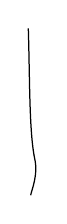
\begin{tikzpicture}[x=1cm,y=1cm]\draw[line width=.45pt] (0,0) .. controls (.02,-.65) and (.01,-1.3) .. (.08,-1.65) .. controls (.13,-1.86) and (.04,-2.06) .. (.03,-2.12);\end{tikzpicture}}

On écrit $F=F_0\amalg G$, et on applique \unsure{lemme|Lemme}

\deleted{\uline{Corollaire 2} Soit $(F_i)_{\unsure{j|i}\in I}$ une famille de composantes connexes deux à deux disjointes. Alors} \deleted{$F=\coprod F_i$} \deleted{la figure engendrée par les $F_i$ est leur somme disjointe $\coprod F_i$} \deleted{et} \deleted{$\subset F$, et si la famille est finie (p. ex. $F$} \deleted{fini} \deleted{figure finie) alors $F=(\coprod F_i)\amalg H$.}

\deleted{Il n'est pas évident que tte figure non vide ait une composante connexe,} \deleted{la difficulté étant dans l'\unsure{existence} \unsure{ou}} \deleted{\unsure{à} des sous-figures \unsure{``compl. dis''|``complém.res''|``comprises''}} \deleted{\inserted{Mais c'est vrai pour les figures de t.f., et a fortiori pour les figures finies. Les}}

\uline{Proposition} Soit $F$ une figure, $A=\overline F\inserted{\subset M}$ l'ens de ses strates. \deleted{Alors l'application} Pour qu'une sous-figure \deleted{$F$} $F_0$ de $F$ soit une comp. conn. de $F$, il f et s que $\overline{F_0}$ soit une composante connexe de l'ens ordonné $A$ (pour l'ordre induit par $\leq$). On trouve ainsi une corr. biunivoque entre l'ens des comp. conn.

\scanpage{64}\mspage{63}
de $F$, et celles de $A$. De plus, $F$ est somme directe disjointe de ses comp. connexes, i.e. $F=\mathop{\mathrm{Sup}}\limits_i F_i$, les comp. connexes $F_i$ deux à deux disjointes\ldots .

% slanted
\margin{\uline{NB} Dans tout ceci, on n'a pas besoin de $C_3$}

\uline{Composantes connexes de \deleted{$\mathcal F$}la \unsure{contrée|contr.} $\mathcal F$.}

Soit $M=\coprod_{i\in I}M_i$ la décomposition de $M$ en composantes connexes.

Pour toute figure $F$, posons
\[
F_i=\mathop{\mathrm{Sup}}\limits_{X\in M_i\cap M_{\leq F}}X
\]
% slanted
\margin{On appelle $F_i$ la \deleted{\unsure{$F_i$}} $i$-composante de $F$, ou la trace de $F$ sur $M_i$ (ou sur $\mathcal F_i$)}

Alors $F$ est la somme directe des $F_i$, \deleted{et \unsure{?}} Si $F$ est de t.f. \inserted{(ou $I=\pi_0(M)$ fini!)} alors tous les $F_i$ sauf un nb fini \unsure{sont|\deleted{sont}} $\varnothing$.
\margin{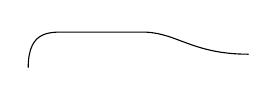
\begin{tikzpicture}[x=1cm,y=1cm]\draw[thin] (0,-.45) .. controls (0,.05) and (.3,0) .. (.55,0) -- (1.5,0) .. controls (1.9,-.02) and (2.1,-.28) .. (2.8,-.28);\end{tikzpicture}}

\deleted{\unsure{Inscrivons|Inversement}} Soit $\mathcal F_i$ l'ens des $F\in\mathcal F$ telle que $\overline F\subset M_i$. Alors \deleted{\unsure{si}} $\mathcal F_i$ satisfait les conditions $C1,C2$\deleted{$,C3$} (et $C3$ aussi, si $\mathcal F$ y satisfait), et $M_i$ est l'ens de ses objets irréductibles.

\deleted{et l'application}
\diagram{\begin{tikzcd}[ampersand replacement=\&,column sep=large,row sep=small,
execute at end picture={\draw[thin,rounded corners=3pt] (oldfamily.south west) -- (oldfigure.west) -- (oldtail.east) .. controls +(right:5pt) and +(right:6pt) .. (oldtail.north east) -- (oldproduct.south west);}]
|[alias=oldfamily]| \mathcal F \arrow[r] \& |[alias=oldproduct]| \prod\mathcal F_i \\
|[alias=oldfigure]| \deleted{F} \arrow[r,mapsto] \& |[alias=oldtail]| \deleted{(F_i)_{i\in I}\ \text{\unsure{ou|où} }F_i\ \text{est le}}
\end{tikzcd}}
Si $F\in\mathcal F$, si $F_i$ sont ses composantes suiv. les $M_i$, alors $\overline{F_i}=\overline F\cap M_i$, $\overline F=\deleted{\coprod}\mathop{\bigcup}\limits_i\overline{F_i}$ (réunion disj)

Pour $i$ fixé, l'application $F\longrightarrow F_i$ commute aux \inserted{Sup quelc., et aux Inf non vides}
\margin{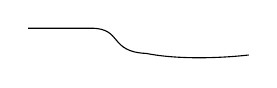
\begin{tikzpicture}[x=1cm,y=1cm]\draw[thin] (0,0) -- (.8,0) .. controls (1.2,0) and (1.02,-.3) .. (1.5,-.32) .. controls (1.9,-.4) and (2.45,-.38) .. (2.8,-.34);\end{tikzpicture}}

L'application
\diagram{\begin{tikzcd}[ampersand replacement=\&,column sep=large]
\mathcal F \arrow[r] \& \prod\mathcal F_i \& F \arrow[r,mapsto] \& (F_i)
\end{tikzcd}}
est injective, et la relation d'ordre de $\mathcal F$ est induite par l'ordre produit
